\documentclass{article}


\usepackage{graphicx}
\usepackage{pdflscape}
\usepackage{minted}
\usepackage{multirow}
\usepackage[colorlinks = true,
            linkcolor = blue,
            urlcolor  = blue,
            citecolor = blue,
            anchorcolor = blue]{hyperref}
\usepackage{geometry}

\usepackage{siunitx}  % for table column alignment


\renewcommand{\thepage}{S\arabic{page}}
\renewcommand{\thesection}{S\arabic{section}}
\renewcommand{\thetable}{S\arabic{table}}
\renewcommand{\thefigure}{S\arabic{figure}}
%\renewcommand{\figurename}{S}


\title{%
    Supplemental Information for \\ 
    \large Interdependent Diffusion: \\ 
    The social contagion of interacting beliefs
    }
\author{James Houghton}


\geometry{margin=0.75in}


\begin{document}

\maketitle
\tableofcontents

\section{Simulation}

\subsection{Simulation code}
The simulations presented in this paper can be replicated with the following code. This code is optimized for clarity over speed. This code was originally written using:
\begin{itemize}
  \item Python 3.7.1
  \item NetworkX 2.3
  \item Pandas 0.24.2
  \item Scikit-learn 0.20.1
\end{itemize}

In this code, \texttt{g} is the social network (a networkx graph object) with \texttt{n} agents. Each node in \texttt{g} is an agent numbered $0$\ldots$n-1$, and has an attribute \texttt{M} which stores the agent's current belief set as a knowledge graph (another networkx graph object for each agent). In the independent condition, agents also have an attribute \texttt{S} representing their susceptibility to beliefs, also formatted as a knowledge graph. When beliefs are passed between functions, it is either as an ordered tuple representing the edge in a knowledge graph \texttt{(2, 7)} or as a numpy array of tuples \texttt{np.array([(2, 7), (2, 16), \ldots])}

To import this module into another python file or jupyter notebook, call:
\begin{minted}{python}
    from example_code import *
\end{minted}
To run a matched simulation of interdependent and independent diffusion, call:
\begin{minted}{python}
    result = run()
\end{minted}
To run a number of simulations and average their output, call:
\begin{minted}{python}
    n_sims = 10
    df = pd.concat([run() for i in range(n_sims)])
    result = df.groupby(level=0).aggregate('mean')
\end{minted}    
This code and supporting materials are available at: \url{https://github.com/JamesPHoughton/interdependent-diffusion}.



~
\hrule


\begin{minted}[linenos]{python}
"""
example_code.py
James Houghton
houghton@mit.edu
"""
import networkx as nx
import numpy as np
import itertools
import pandas as pd
import copy
from sklearn.decomposition import PCA


def susceptible(g, agent, belief):
    """Assess whether an agent is susceptible to a given belief"""
    if 'S' in g.node[agent]:  # has exogenous susceptibility defined (independent case)
        return g.node[agent]['S'].has_edge(*belief)
    else:  # interdependent case
        try:
            return nx.shortest_path_length(g.node[agent]['M'], *belief) <= 2  
            # current holders are also susceptible
        except (nx.NetworkXNoPath, nx.NodeNotFound):
            return False  # no path exists between the nodes


def adopt(g, agent, belief):
    """Assess whether an agent will adopt a given belief"""
    suscep = susceptible(g, agent, belief)
    exposed = any([belief in g.node[nbr]['M'].edges() for nbr in g[agent]])
    return suscep and exposed  # both susceptibility and exposure required to adopt


def measure(g, beliefs, initial_susceptible=None, initial_adopted=None):
    """Take measurements of the state of the system (for creating figures)"""
    res = {}  # dictionary to collect measurements

    # Fig 2A: Susceptible and adopting populations
    # --------------------------------------------
    # build a matrix of who (rows) is susceptible to what beliefs (columns)
    suscep = pd.DataFrame(index=g.nodes(), columns=[tuple(b) for b in beliefs])
    for agent in g:
        for belief in suscep.columns:
            suscep.at[agent, belief] = susceptible(g, agent, belief)
    # return average susceptible fraction across all beliefs
    res['% susceptible'] = suscep.mean().mean()  

    # build a matrix of who (rows) holds what beliefs (columns)
    adopt = pd.DataFrame(index=g.nodes(), columns=[tuple(b) for b in beliefs])
    for agent in g:
        for belief in adopt.columns:
            adopt.at[agent, belief] = g.node[agent]['M'].has_edge(*belief)
    # return average adopting fraction across all beliefs
    res['% adopted'] = adopt.mean().mean()  

    # Fig 2B:correlation between predicted new adoption and actual new adoption
    # -------------------------------------------------------------------------
    if initial_adopted is not None and initial_susceptible is not None:  # t>0
        res['initial prediction correlation'] = np.corrcoef(
            adopt.sum(axis=0) - initial_adopted,
            initial_susceptible - initial_adopted
        )[1, 0]  # select an off-diagonal term
    else:  # first time => establish baseline
        initial_adopted = adopt.sum(axis=0)
        initial_susceptible = suscep.sum(axis=0)
        res['initial prediction correlation'] = np.nan  # measure has no meaning at t0

    # Fig 2C: correlation between a belief and it's most popular neighbor
    # -------------------------------------------------------------------
    adopt_counts = pd.DataFrame()
    adopt_counts['self'] = adopt.sum(axis=0)
    adopt_counts['leading neighbor'] = 0
    for c1 in adopt.columns:
        # search for the leading neighbor's popularity
        leading_value = 0
        for c2 in adopt.columns:
            if len((set(c1) | set(c2))) == 3:  # three nodes total => c1 and c2 are neighbors
                leading_value = max(leading_value, adopt_counts.loc[[c2], 'self'].values[0])
        adopt_counts.at[[c1], 'leading neighbor'] = leading_value
    res['leading neighbor correlation'] = adopt_counts.corr().loc['self', 'leading neighbor']

    # Fig 2D: clustering coefficient of 10% most popular beliefs
    # ----------------------------------------------------------
    # shuffle within sorted value so that when 10% falls within a level of popularity
    # we don't add spurious clustering by selecting sequential beliefs
    adopt_counts['shuffle'] = np.random.rand(len(adopt_counts))
    adopt_counts.sort_values(by=['self', 'shuffle'], inplace=True, ascending=False)
    leaders = adopt_counts.iloc[:int(len(adopt_counts) * 0.1)]  # take leading 10% of beliefs
    # construct knowledge graph from leading beliefs
    popular_graph = nx.from_edgelist(list(leaders.index))  
    res['popular belief clustering'] = nx.average_clustering(popular_graph)

    # Fig 3A: similarity btw 5% and 95% most similar pairs
    # ----------------------------------------------------
    n_agents = len(adopt.index)
    trimask = np.tri(n_agents, n_agents, 0, dtype='bool')  # mask the diagonal and below
    corrs = adopt.astype(float).T.corr().mask(trimask).stack()
    res['95% similarity'] = np.percentile(corrs, 95)
    res['5% similarity'] = np.percentile(corrs, 5)

    # Fig 3B: PC1 percent variance
    # ----------------------------
    pca = PCA(n_components=1)
    pca.fit(adopt)
    res['PC1 percent of variance'] = pca.explained_variance_ratio_[0] * 100

    return res, initial_susceptible, initial_adopted


def simulate(g, n_steps=10):
    """Conduct a single run of the simulation with a given network"""
    # capture a list of all the beliefs in the population
    beliefs = np.unique([tuple(sorted(belief)) for agent in g 
                         for belief in g.node[agent]['M'].edges()], axis=0)

    # measure initial conditions
    m0, initial_susceptible, initial_adopted = measure(g, beliefs)  
    # initialize list to collect measurements at each time step
    m = [m0]  

    # perform the simulation
    for step in range(n_steps):  
        # cycle through agents in random order
        for ego in np.random.permutation(g):  
            # cycle through all possible beliefs in random order
            for edge in np.random.permutation(beliefs):  
                # check whether the selected agent adopts the selected belief
                if adopt(g, ego, edge):  
                    # add the belief to the agent's knowledge graph
                    g.node[ego]['M'].add_edges_from([edge])  
        # ignore returned init suscep and adopt            
        m.append(measure(g, beliefs, initial_susceptible, initial_adopted)[0])  

    return pd.DataFrame(m)  # format as pandas DataFrame


def run(n_agents=60, deg=3, n_concepts=25, n_beliefs=25, t_match_susceptibility=0, n_steps=10):
    """
    Run a matched pair of simulations (inter/independent) from the same initial condition

    Parameters
    ----------
    n_agents: (integer) - Number of agents in the population
    deg: (integer) - How many neighbors each agent has (on average)
    n_concepts: (integer) - How many nodes are in the complete semantic 
                            network that beliefs are drawn from
    n_beliefs: (integer) - Exact number of beliefs (semantic net edges) 
                           each agent is initialized with
    t_match_susceptibility: (integer) - time step at which the interdependent 
                                        susceptibility will be matched
                                        (must be less than n_steps)
    n_steps: (integer) - Number of time steps in the simulation
    """

    # Shared Initial Setup
    # --------------------
    # create a random connected social network g0
    connected = False
    while not connected:
        g0 = nx.gnm_random_graph(n=n_agents, m=int(n_agents * deg / 2))
        connected = nx.is_connected(g0)

    # give agents their initial beliefs
    nx.set_node_attributes(
        g0,
        name='M',  # set node attribute 'M' (for 'mind')
        # create a knowledge graph with a different random set of beliefs
        # for each agent, and assign to nodes in the social network
        values={agent: nx.gnm_random_graph(n_concepts, n_beliefs) for agent in g0}
    )

    # Interdependent simulation
    # -------------------------
    g1 = copy.deepcopy(g0)  # create copy, to preserve initial conditions for other case
    res1 = simulate(g1, n_steps)

    # Independent simulation
    # ----------------------
    g2 = copy.deepcopy(g0)  # copy from original starting conditions

    # calculate the population likelihood of being susceptible to a given (non-held) belief
    p = ((res1.loc[t_match_susceptibility, '% susceptible'] - res1.loc[0, '% adopted']) /
         (1 - res1.loc[0, '% adopted']))

    # choose a set of beliefs for each agent to be susceptible to
    new_sus = {}
    for agent in g2:
        # potentially susceptible to any belief
        gc = nx.complete_graph(n_concepts)  
        # temporarily remove existing beliefs
        gc.remove_edges_from(g2.node[agent]['M'].edges())  
        # from remainder, randomly select a subset of beliefs to be susceptible to
        edges = list(itertools.compress(
            list(gc.edges()),  # selection candidates
            np.random.binomial(n=1, p=p, size=len(gc.edges())) == 1  # selection mask
        ))
        # add susceptibility to existing beliefs
        edges += list(g2.node[agent]['M'].edges())  
        # create networkx graph of susceptibilities
        new_sus[agent] = nx.from_edgelist(edges)  

    # assign new susceptibilities to positions in social network
    nx.set_node_attributes(g2, name='S', values=new_sus)  
    
    # perform independent simulation
    res2 = simulate(g2, n_steps)  

    return pd.merge(res1, res2, left_index=True, right_index=True,
                    suffixes=(' (inter)', ' (indep)'))  # format as single DataFrame

\end{minted}

\hrule

\subsection{Motivating the ``Knowledge Graph'' representation of belief interaction}
There are two primary ways that we could model the interaction between beliefs. One method used by Friedkin et al. \cite{friedkin2016network} is to create a matrix of the compatibility between candidate beliefs (rows) and preexisting beliefs (columns). In this model, weights in the matrix determine the influence of (unstructured) existing beliefs on the probability of an individual adopting each candidate belief. This formulation assumes external `logic' under which certain beliefs naturally go together. 

A second method is the knowledge graph representation suggested by Goldberg and Stein \cite{goldberg2018beyond} and by Schilling \cite{schilling2005small}, in which existing beliefs have no independent effect on an an agent's susceptibility to a candidate belief. Instead, they influence future adoption decisions through the structure they create in the individual's knowledge graph. In this representation, all beliefs are potentially compatible with one another, depending on the arrangement of other beliefs that the individual holds.

When we study the effect of diffusion on the emergence of worldviews and polarization, it's important that we choose a representation of belief interaction that does not foreordain particular outcomes. If we can predict patterns of belief clustering and polarization from the decision logic alone, then the simulation will be unable to identify whether clustering is shaped by social contagion, or is merely a result of the assumed decision logic.

Unfortunately, an interdependence matrix which maps the presence of belief A to the likelihood of adopting belief B will always be informative of the final configuration of beliefs (or trivial). We can demonstrate this outcome with an extremely simple deterministic model with no diffusion at all. This model is in the style of Friedkin et al.\cite{friedkin2016network}, but omits social influence, stochasticity, and degrees of belief. These simplifications let us see intuitively why the interdependence matrix is problematic for our purpose. When stochasticity, social influence, etc. are present, the problem doesn't go away, it is just masked by the complexity of the model. In this simplified interdependence-matrix belief adoption model:

\begin{enumerate}
    \item Each agent is exposed to all beliefs in every timestep (making this an individual learning model, not a social learning model).
    \item The presence of belief ‘A’ in an agent's existing belief set either contributes (+) to an agent's likelihood of adopting candidate belief ‘B’, or takes away from it (–).
    \item The absence of belief ‘A’ from an agent's belief set has no direct influence on an agent's likelihood of adopting candidate belief ‘B’.
    \item Belief adoption is binary and permanent.
    \item Agents adopt a candidate belief if the majority of their current beliefs support doing so.\footnote{Other thresholds would lead us to the same insights that we will develop with the ``majority rule''.}
\end{enumerate}

To show that the matrix of influence is informative of the outcomes of contagion, we simulate a population of 64 individuals, each with a unique combination of six beliefs, denoted A-F. The top center chart in Fig. \ref{fig:rule_matrix} illustrates this starting condition. Each column represents an individual agent (0-63), each row represents a belief (A-F). I darken the corresponding square to show that an agent has adopted a particular belief. To the right-hand side of the adoption plot, a histogram shows the total number of individuals adopting each belief. In the initial condition, all beliefs have been adopted by 32 individuals.

\begin{figure}[h!]
\centering
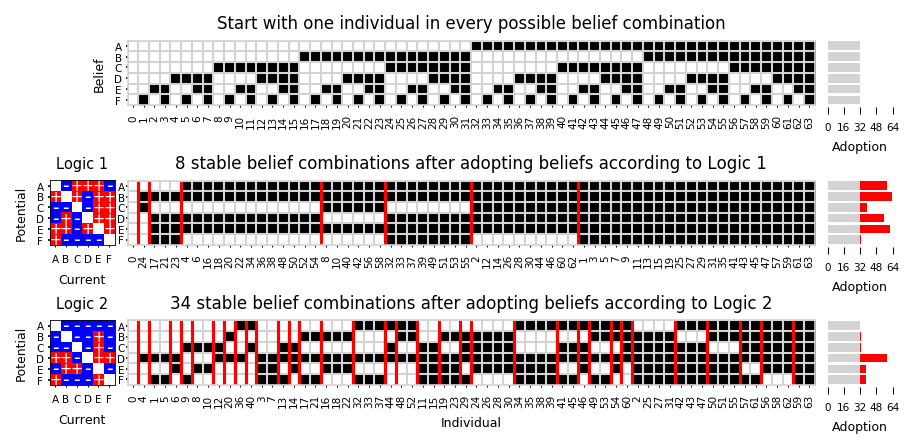
\includegraphics[width=1.0\columnwidth]{rule interdependence matrix.png}
\caption{With an interdependence-matrix style belief structure, polarization and belief clustering can be explained by the assumed compatibility relationships. But where does this logic come from?}
\label{fig:rule_matrix}
\end{figure}

The subsequent two plots in Fig. \ref{fig:rule_matrix} show the final adoption of beliefs under two influence matrices (Logic 1 and Logic 2) in the style of Friedkin et al.\cite{friedkin2016network}. Logic 1 and Logic 2  are randomly generated influences between beliefs, shown as + (red) and – (blue). In each matrix, if an individual holds A, then the influence of that belief on the adoption of belief B is found in Column A, Row B. In Logic 1, the influence of A on B is positive, and in Logic 2, this influence is negative. 

For each individual, we calculate the net influence of existing beliefs on adoption of each candidate belief. If the candidate belief gets a majority of + votes then it is adopted. We repeat the process until all agents have converged on a stable combination of beliefs. 

Any model of social learning with binary and permanent belief adoption and a finite number of beliefs will show some form of belief consolidation, and an increase in mean similarity between individuals. We expect to see that from our maximally-differentiated initial conditions, some groups of stable belief combinations should emerge. In the adoption plots in Fig. \ref{fig:rule_matrix}, I group individuals according to their stable sets of beliefs, indicating the groups with a red divider.

Despite being drawn from the same pool of possible logics, the two Friedkin-style logics yield very different stable combinations of beliefs. In Logic 1, there are 8 different stable combinations, and in Logic 2, there are 34. In a diffusion model, we would expect to see a lot more consolidation of beliefs, and clustering of individuals, using Logic 1 rather than Logic 2, regardless of social contagion. Moreover, the two different logics strongly influence which beliefs we should expect to be widely adopted in the population. Logic 1 suggests strong new adoption (shown in red) of beliefs A, B, D, and E. Logic 2 shows that only belief D is widely adopted, with belief A having no new diffusion at all.

In the real world, it may well be that a natural logic ties some beliefs together, and promotes the diffusion of some beliefs at the expense of others. In our simulation, however, this influence makes it difficult to identify clustering and amplification of beliefs that is due to social contagion. In this paper, I have suggested an alternative formulation, in which beliefs are formalized as edges in a knowledge graph, and the adoption rule is that beliefs are adopted if they close a triangle in an individual’s knowledge graph.

In Fig \ref{fig:rule_triangle}, I repeat the above analysis with this new formulation. Again there are six beliefs, representing all of the possible edges in a knowledge graph with concepts P, Q, R and S. Again, each of 64 individuals is initialized with a unique combination of beliefs, and has access to all six beliefs. Each individual adopts new beliefs that are consistent with the triangle-closing decision rule, and I plot the stable belief combinations after each individual has individually converged. As there is only one decision rule, there can be only one outcome for grouping the sets of stable beliefs.  


\begin{figure}[h!]
\centering
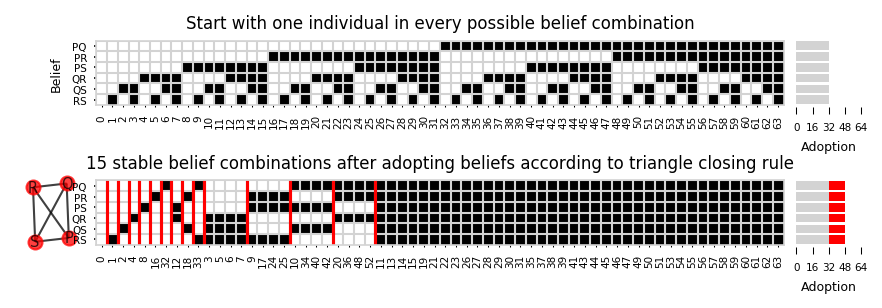
\includegraphics[width=1.0\columnwidth]{rule triangle closing.png}
\caption{With the knowledge graph representation of belief structure, we have confidence that any variance in adoption patterns, or differences in social clustering, are due to the interaction of the belief structure with the diffusion process.}
\label{fig:rule_triangle}
\end{figure}

With this formalization, we know exactly how the decision rule for adoption influences the number of possible stable states; and most importantly, these states are symmetric with respect to the individual beliefs. The histogram to the right of the second row of \ref{fig:rule_triangle} shows that each belief has an equal number of new adoptions, and that we should not expect any beliefs to preferentially diffuse as a result of the decision rule itself. 

In this paper I have shown that some beliefs do indeed diffuse much more widely than others, and that the population clusters into a subset of the possible stable states. Because the decision rule does not influence which of the beliefs diffuse most widely, or suggest variation in the number of social clusters we can expect, we have confidence that the results are genuinely due to the interactions between beliefs as they diffuse.


\subsection{Sensitivity to parameters}
\label{section:thresholds}
Figure 2D in the main body of the paper makes a comparison between the clustering coefficient amongst the most popular beliefs, defined as the 10\% most widely adopted. Fig. \ref{fig:clustering_threshold} in this supplement shows that the qualitative result is insensitive to this particular choice of threshold between approximately 5\% and 40\%.

\begin{figure}[h!]
\centering
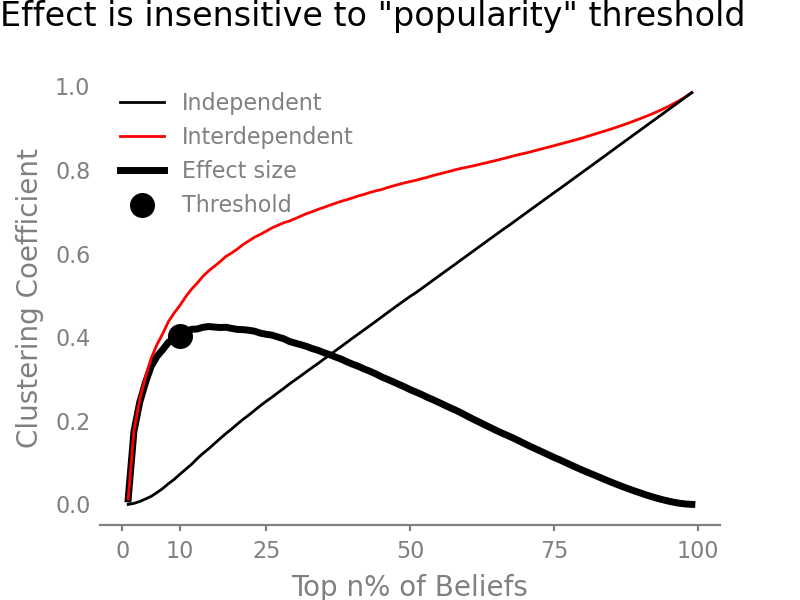
\includegraphics[width=0.5\columnwidth]{insensitive_to_popularity_threshold.png}
\caption{The effect of interdependence on the clustering of the most popular beliefs is robust to a wide range of thresholds for ``popularity''. In the simulations presented in this experiment, I use a conservative 10\% threshold.}
\label{fig:clustering_threshold}
\end{figure}

In Fig. 3A, 5B and 5C of the paper, I use 5\textsuperscript{th} and 95\textsuperscript{th} percentile values to characterize the level of similarity across and within ideological camps. These thresholds are arbitrary, in that we could have plausibly used a wide range of other values. Fig. \ref{fig:camp_threshold} shows that the qualitative effect we are interested in is insensitive to the precise choice of threshold.

\begin{figure}[h!]
\centering
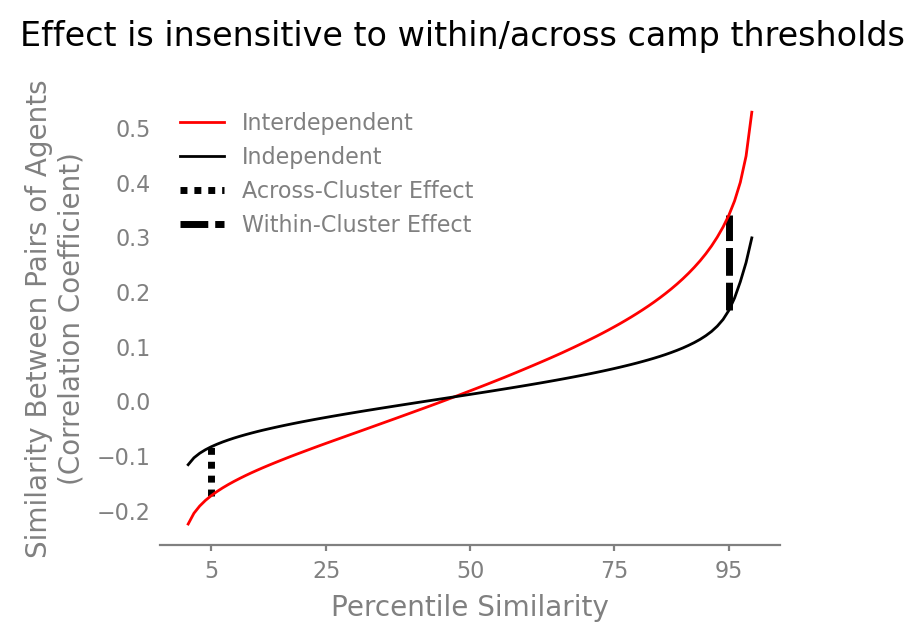
\includegraphics[width=0.6\columnwidth]{insensitive_to_camp_thresholds.png}
\caption{The effect of interdependence on within-camp and across-camp similarity is robust to a wide range of thresholds for assessing whether relationships are within or across camp. In the simulation and experiment, I use conservative 5\textsuperscript{th} and 95\textsuperscript{th} percentile thresholds.}
\label{fig:camp_threshold}
\end{figure}

\section{Analysis of Observational Data}

\subsection{Description of Datasets}
All code needed to generate Fig. 4 in the main body is available in the \href{https://github.com/JamesPHoughton/interdependent-diffusion/tree/master/observational}{/observational} folder of the code repository.

\subsubsection{KPTimes}
The KPTimes dataset \cite{gallina-etal-2019-kptimes} contains New York Times articles between January 1, 2006 and June 25, 2019. The analysis in Fig. 4 of the main body included 288,545 documents from 27 categories. These categories were selected on the criteria that they include $>= 3000$ documents. When a document was labeled with multiple categories, it was assigned to the smallest category with $>= 3000$ documents. The categories included in the analysis are: (parentheses indicate the number of documents per category) 

\noindent
\texttt{africa (5203), americas (4801), asia (16218), baseball (12754), basketball (7023), business (33686), dealbook (3815), economy (3186), europe (14630), football (8209), global (5762), golf (3471), hockey (4323), media (9427), middleeast (12338), national (3513), ncaabasketball (4011), ncaafootball (3180), nyregion (43221), politics (15094), science (7419), soccer (5254), sports (15059), technology (9634), tennis (3520), us (29420), world (4374)}

\subsubsection{Web of Science}
The Web of Science dataset \cite{WOSv6} was originally collected by Kowsari et al. \cite{kowsari2017HDLTex} for training text classification algorithms, and was repurposed for this analysis. The datset contains 46,985 documents in 7 Major fields: (parentheses indicate the number of documents per category)

\noindent
\texttt{Computer Science (6514), Civil Engineering (4237), Electrical Engineering (5483), \\Mechanical Engineering (3297), Medical (14625), Psychology (7142), Biochemistry (5687)}


\subsubsection{Pew Political Typology Survey}
The Pew Political Typology Survey interviewed 10,013 US adults in three approximately equal waves from January 23, 2014 through March 16, 2014. Each wave was split into half land-line and half cellphone interviews. The analysis in Fig. 4 of the main body included 58 questions about political opinions, chosen prior to data observation to focus only on political opinions (i.e. to exclude questions about demographics and other ascribed characteristics) and to consolidate redundant questions. Not all questions were included in each wave. The question codes included are:

\noindent
\texttt{q25a, q25b, q25c, q25d, q25f, q25g, q25h, q25i, q25j, q25k, q25l, q25m, q25n, q25o, q25p, q50q, q50r, q50s, q50t, q50u, q50v, q50w, q50y, q50z, q50aa, q50bb, q50dd, q50ee, q50ff, q50gg, q50hh, q51ii, q51jj, q51kk, q51ll, q51mm, q51oo, q51pp, q53, qb26, qc26, qb106, qb107, qb109, qb110, qc115, qc116, q121, q122, q123, q124, q125, q126, qc127, qc128, qc135, qc56, qb108}


\subsubsection{World Values Survey}
The 2020 World Values Survey \cite{wvs2020} contains 70,867 responses collected from 2017-2020. The analysis in Fig. 4 of the main body used 144 questions relating to apolitical social values. The questions to be used were chosen prior to data observation to focus only on social opinions (i.e. to exclude questions about demographics and other ascribed characteristics, and to exclude explicitly political questions) and to consolidate redundant questions. The question codes included are:

\noindent
\texttt{Q1, Q2, Q3, Q4, Q5, Q6, Q7, Q8, Q9, Q10, Q11, Q12, Q13, Q14, Q15, Q16, Q17, Q18, Q19, Q20, Q21, Q22, Q23, Q24, Q25, Q26, Q27, Q28, Q29, Q30, Q31, Q32, Q33, Q34, Q35, Q36, Q37, Q38, Q39, Q40, Q41, Q43, Q44, Q58, Q59, Q60, Q61, Q62, Q63, Q64, Q65, Q66, Q67, Q68, Q69, Q70, Q71, Q72, Q73, Q74, Q75, Q76, Q77, Q78, Q79, Q80, Q81, Q82, Q83, Q84, Q85, Q86, Q87, Q88, Q89, Q106, Q107, Q108, Q109, Q110, Q121, Q122, Q123, Q124, Q125, Q126, Q127, Q128, Q129, Q130, Q158, Q159, Q160, Q161, Q162, Q163, Q164, Q165, Q166, Q167, Q168, Q169, Q170, Q171, Q172, Q173, Q174, Q176, Q177, Q178, Q179, Q180, Q181, Q182, Q183, Q184, Q185, Q186, Q187, Q188, Q189, Q190, Q191, Q192, Q193, Q194, Q195, Q196, Q197, Q198, Q235, Q236, Q237, Q238, Q239, Q241, Q242, Q243, Q244, Q245, Q246, Q247, Q248, Q249}

The analysis in Fig. 4 of the main body includes a curve for each of 49 different country codes: (parentheses show number of respondents)

\noindent
\texttt{AND (1004), ARG (1003), AUS (1813), BGD (1200), BOL (2067), BRA (1762), CHL (1000), CHN (3036), COL (1520), CYP (1000), DEU (1528), ECU (1200), EGY (1200), ETH (1230), GRC (1200), GTM (1203), HKG (2075), IDN (3200), IRN (1499), IRQ (1200), JOR (1203), JPN (1353), KAZ (1276), KGZ (1200), KOR (1245), LBN (1200), MAC (1023), MEX (1739), MMR (1200), MYS (1313), NGA (1237), NIC (1200), NZL (1057), PAK (1995), PER (1400), PHL (1200), PRI (1127), ROU (1257), RUS (1810), SRB (1046), THA (1500), TJK (1200), TUN (1208), TUR (2415), TWN (1223), UKR (1289), USA (2596), VNM (1200), ZWE (1215)}

\subsection{Alternate clustering analysis}
The analysis presented in Fig. 4A of the main body included connections between all keywords attached to each newspaper article or academic paper. An alternate method of producing these graphs is to only include connections between \textit{pairs} of keywords within each article, randomly selected without replacement. While this results in a significantly sparser dataset, it guarantees that none of the clustering observed is due to clustering within documents. 

With this method, the overall clustering is reduced across all thresholds, and in particular thresholds that include keywords found in only a few documents. However, the qualitative prediction of increased clustering among the most popular connections between keywords remains, as shown in Fig. \ref{fig:pairwise_clustering}.

\begin{figure}[H]
\centering
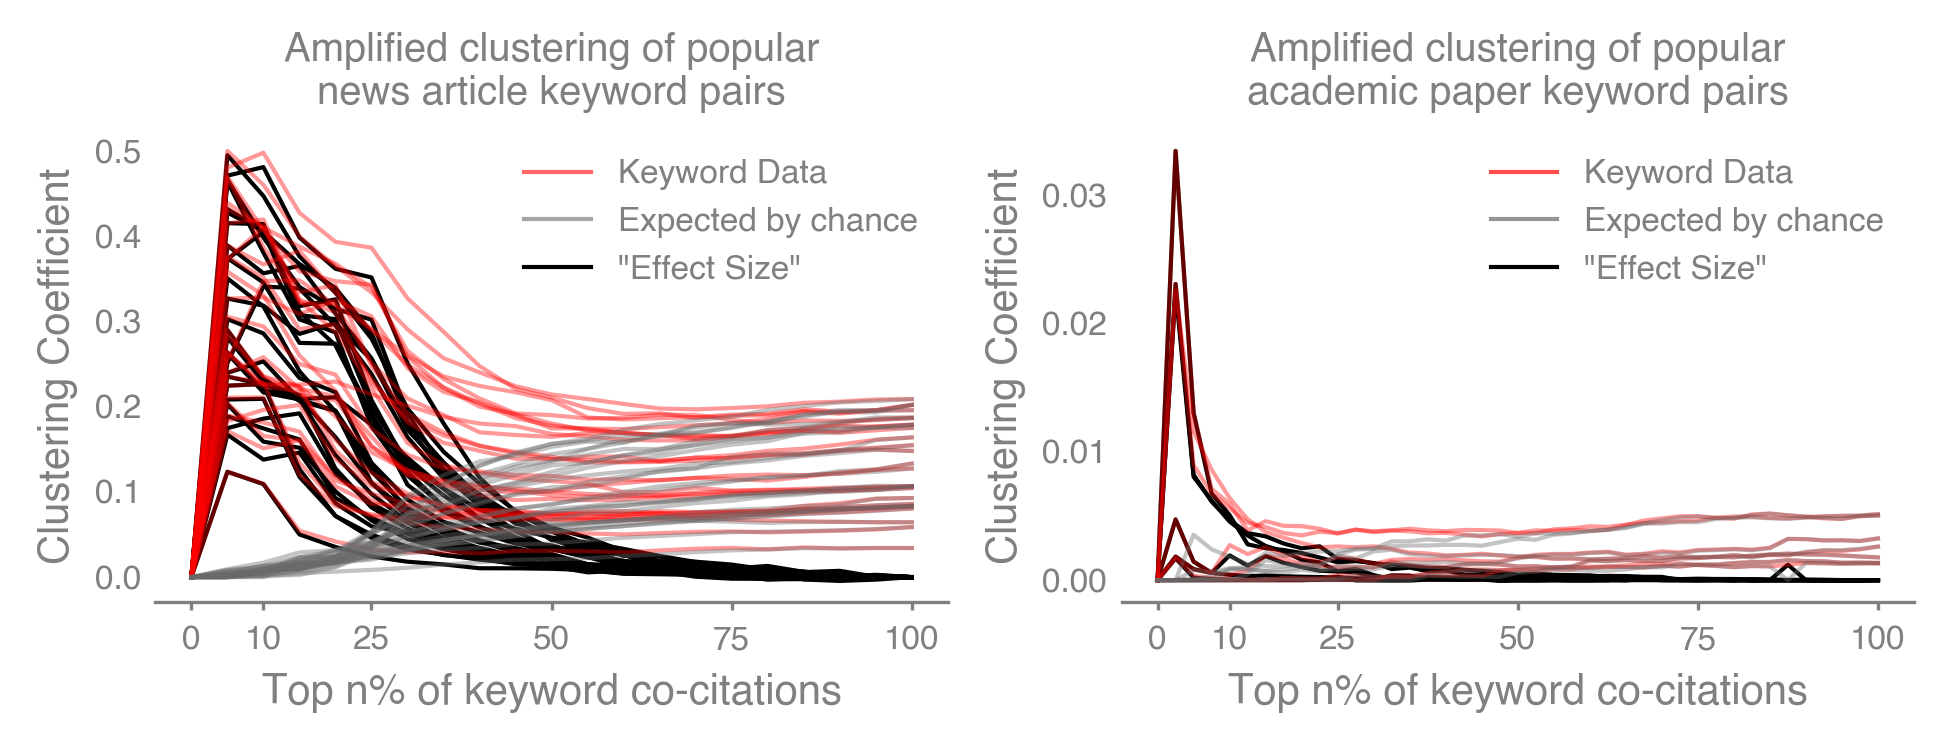
\includegraphics[width=0.8\columnwidth]{Pairwise_Clustering.png}
\caption{The predicted amplification of clustering among popular keyword pairs is preserved when the data is restricted to disallow any contribution to clustering from the attachment of more than two keywords to the same article.}
\label{fig:pairwise_clustering}
\end{figure}


\section{Experiment}
The experimental design had two major objectives. 1) Allow for the manipulation of interdependence between diffusants, and 2) minimize the spillover of real-world polarization into the artificial social networks of the experiment. Beyond those considerations, I wanted to use a set of diffusants that individuals could quickly understand and would be interested in. A detective case solving a burglary was sufficiently relatable and abstract from the real world to serve as a stimulus and manipulation. Section \ref{design_considerations} details the various experiment design choices that were not specific to the manipulation. Section \ref{interface} details the participant's experience, and Section \ref{manipulation} details the design of the mystery's clues, which formed the experimental manipulation. Section \ref{data_collection} describes how data was collected and handled. Section \ref{prereg} describes the experiment's preregistration and deviations between the preregistration and the realized experiment. Section \ref{outcomes} lists outcomes of the experiment that have not already been discussed. 




\subsection{Design considerations and experiment parameters}
\label{design_considerations}
There are many ways that the game interface and experimental parameters could have been implemented. Each decision took into account the feasibility of implementation, the constraints of the online lab context, the desire to create a naturalistic information and task environment, and the desire to cleanly isolate the mechanisms being tested. Below I justify the major decision points.

\textbf{Information was presented to each participant all at once} in the form of Detectives' Notebooks shared by their neighbors. This was an intuitive structure for the detective-game task; it allowed players to quickly understand how their categorization decisions would be shared and how the information was presented to them. There is a slight cost in real-world representativeness with this design choice, as it is different from how information is typically presented in social media. However, the alternative ``scrolling feed'' type information display has recency and primacy effects, and opens questions about how we should aggregate social information from multiple players. Showing all information at once, in the same order that it is sorted by the neighbor, eliminates the effect of alternate ordering sequences.

\textbf{Individuals had three social network neighbors.} 
Given the chosen display, the number of neighbors is limited by the size of the screen and an individual’s ability to process information. The minimum number of neighbors for a non-trivial social network is 3, and is also a reasonable number for managing the cognitive load in the game.

\textbf{Individuals began with four clues in their detectives' notebooks.}
Fewer starting clues are preferred for minimizing individuals' cognitive load. With three neighbors, individuals began the game having to process 16 clues. The next increment (5 starting clues each) would have given 20 items for an individual to process at game start, which (in ``friends and family'' beta tests) proved to be cognitively overwhelming.

\textbf{The social network contained 20 players.}
Larger numbers of players are better for generalizability and seeing an effect size. On the other hand, smaller networks allow more replications and are easier to recruit and coordinate. There needed to be enough players that the mean shortest-path-length was greater than two, to realistically represent multi-stage diffusion. Pilot tests showed that we could reasonably expect to fill four 20-player games at once, and simulation suggested that 20-player networks should be sufficient to detect an effect size.

\textbf{The social networks were shaped as a dodecahedron and a regular connected caveman (k=5) network.}
I evaluated eleven symmetric candidate social networks (n=20, degree=3) shown in Fig. \ref{fig:all_networks}. Of this set, the dodecahedral network minimizes the average shortest path between individuals with no network clustering, and represents a social network in which \textit{a priori} we should expect to see low polarization. A regular connected caveman network maximizes the characteristic path length and exhibits strong clustering, and so we expect to see more polarization in this network. Edgelists for each of the eleven social networks are are available in the \href{https://github.com/JamesPHoughton/interdependent-diffusion/tree/master/experiment/setup}{/experiment/setup} folder of the code repository.

\begin{figure}[h!]
\centering
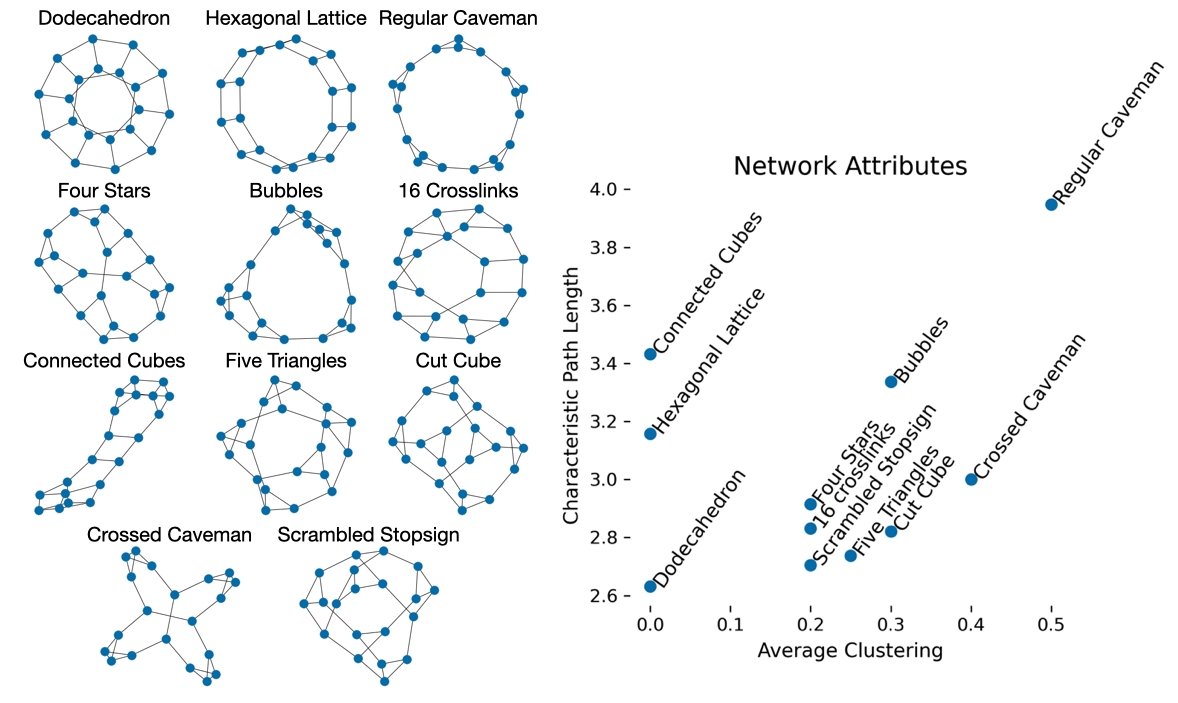
\includegraphics[width=0.9\columnwidth]{All Networks.png}
\caption{Various possible social networks were evaluated, and two were selected (dodecahedron and regular caveman) to maximize the difference in average clustering and characteristic path length.}
\label{fig:all_networks}
\end{figure}

\textbf{Each game contained 78 unique clues.}
From an information diversity perspective, more clues is better. With 4 starting clues and 20 players, we can have up to 80 unique clues in the game. A complete 13 node clue network (knowledge graph) has 78 clues, and the two spots remaining were filled with the (given) link between the crime scene and the stolen object. 

\textbf{Each clue was represented in exactly 1 starting notebook.}
In order to make sure that the initial frequency of information in the network did not bias the network to certain outcomes, each clue was present exactly once in the clues initially assigned to players. Other than this constraint, clues were assigned randomly. The clue linking the stolen object to the crime scene was included 2 additional times to fill out the 80 slots (20 players * 4 starting clues) available.

\textbf{The game was played for 8 minutes.} 
Games needed to be long enough that participants had a chance to sort clues and make sense of the mystery, but short enough that they remained engaged and did not drop out of the experiment. Varying the length of games during pilot trials suggested that 8 minutes was a good balance between these constraints. Fig. \ref{fig:player_activity} shows that the average rate of categorization activity built over the first minute as players started to develop an understanding of the mystery, and then declined as individuals settled in on a solution.

\begin{figure}[h!]
\centering
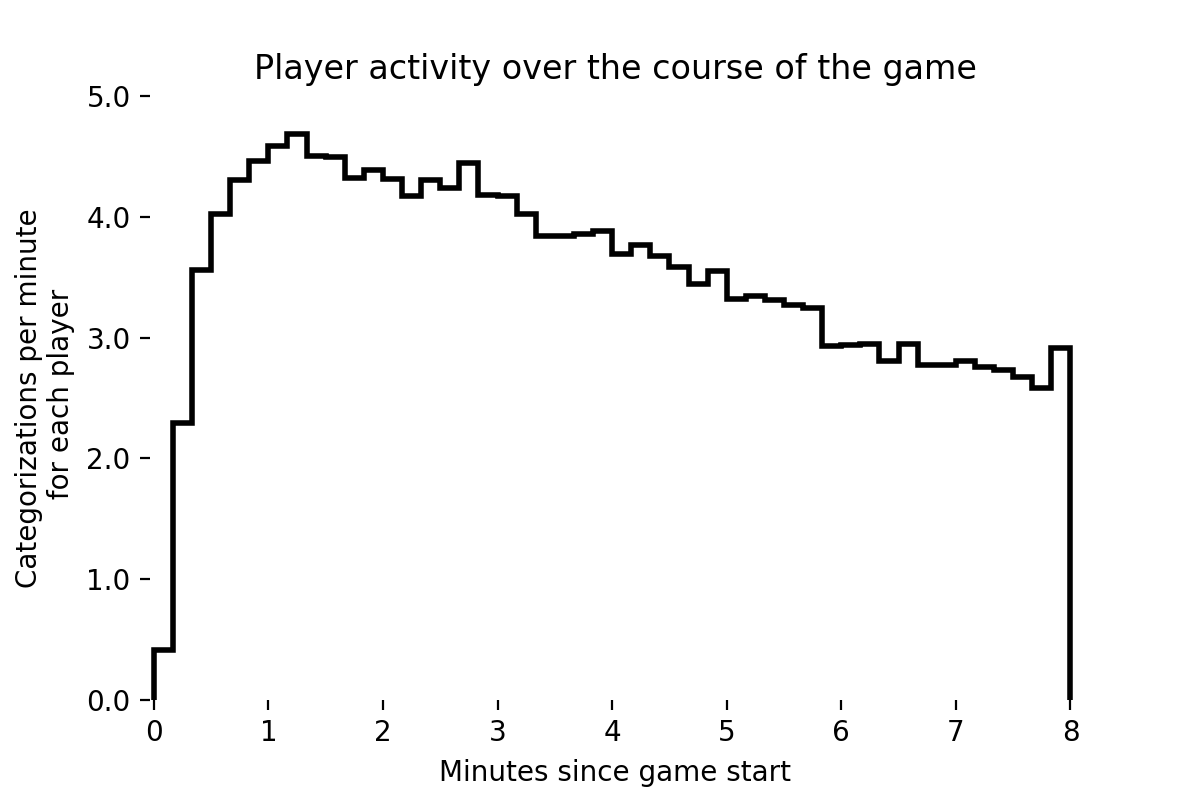
\includegraphics[width=.5\columnwidth]{player_activity.png}
\caption{Average rate of activity for all players in experiment runs (excluding pilots).}
\label{fig:player_activity}
\end{figure}

\textbf{Post-game opinions were elicited as likelihood of participation for each element in the mystery.}
Rather than force individuals to make a discrete choice between suspects/vehicles etc., individuals assessed how likely each element of the mystery was to have been involved in the crime. While this is different from how a jury might assess the guilt of a suspect in a courtroom, it gave more resolution on the strength of individuals' opinions. 

\textbf{Each condition was sampled 30 times.}
Each sample of the four conditions in this experiment cost about \$400. As there is no precedent for this type of multi-player, multi-diffusant experiment, and I did not have enough pilot data to know how effect sizes predicted in simulation would translate to experiment, it was difficult to assess the marginal benefit of additional samples relative to their cost. Based on the technical success of the pilots, I was able to secure \$12,000 to compensate participants, allowing for 30 sets of data-points.

\subsection{Design of participant interface}
\label{interface}
The experiment was implemented using the Empirica \cite{almaatouq2021empirica} framework, a platform for realtime multiparticipant web-based experiments.

\subsubsection{Consent}
Upon arrival, participants were shown a consent screen (Fig. \ref{fig:consent}) telling them about the study and what they would be expected to do, including information that the games were oversubscribed and that they may not be able to complete the whole game. Those who gave their consent to participate continued to training.


\begin{figure}[h!]
\centering
\fbox{
\includegraphics[width=0.6\columnwidth]{01_consent.png}}
\caption{Participants indicate consent before proceeding.}
\label{fig:consent}
\end{figure}

\subsubsection{Training}

The first training screen (Fig. \ref{fig:training1}) instructed participants in how to interact with the Detective Game interface. They were asked to sort clues into ``Promising Leads'' and ``Dead Ends'' by dragging them into labeled sections of their ``Detective’s Notebook''. Having done so, they were shown clues that two artificial ``collaborators'' had categorized as promising leads. Each participant then had to correctly sort the collaborators' clues before they could continue to the next training screen.

\begin{figure}[h!]
\centering
\fbox{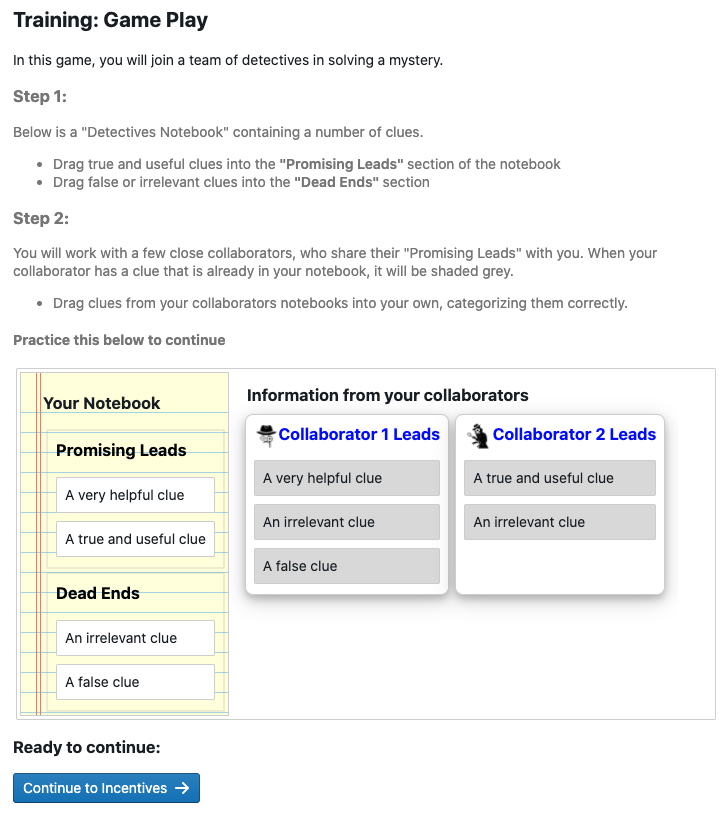
\includegraphics[width=.7\columnwidth]{04_training1c.png}}
\caption{Training screen 1: How to use the game interface}
\label{fig:training1}
\end{figure}

The second training screen (Fig. \ref{fig:training2}) told participants how they would be rewarded for their performance. Individuals were told that they would receive \$0.10 for each clue correctly categorized as a promising lead, and would be penalized \$0.10 for each clue categorized as a promising lead that was actually false. They were also told that they would be rewarded for their team’s average performance, receiving the average of all players’ individual bonuses as a Team Bonus. These incentives encourage individuals to carefully sort each clue according to their best estimate of its veracity, and to share clues with their neighbors that they believe will improve the team’s collective sense-making ability. Setting the reward for success to be equal to the penalty for mistakes encourages participants to accurately assess each statement, rather than ‘hedge’ by keeping too many or too few clues. Participants completed a comprehension check to ensure that they understood their incentives before they could proceed to the game. Participants were compensated \$1 for training.

\begin{figure}[h!]
\centering
\fbox{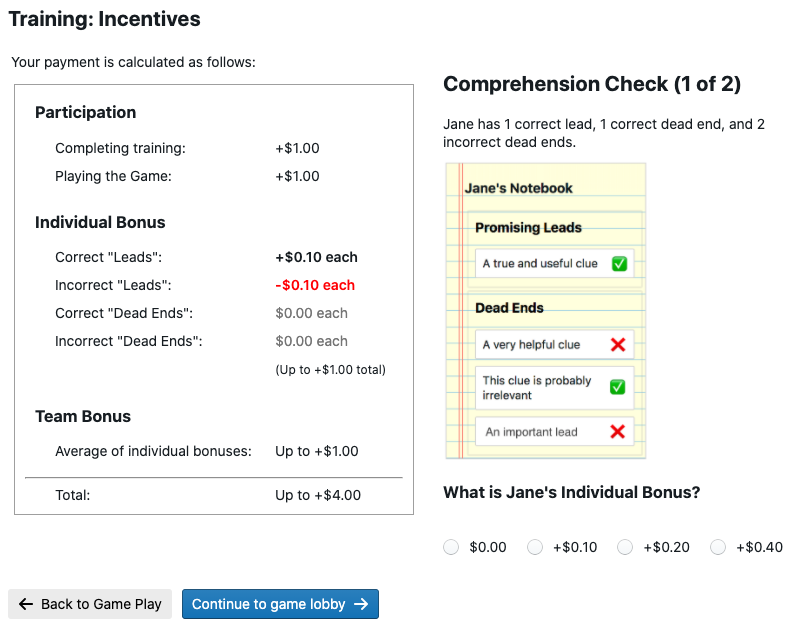
\includegraphics[width=.7\columnwidth]{05_training2a.png}}
\caption{Training screen 2: Incentives and comprehension check}
\label{fig:training2}
\end{figure}

\subsubsection{Game introduction}
After completing training (taking between 2 and 4 minutes), participants entered a waiting room until enough players had completed training and were ready to play.\footnote{Participants in each block were randomized into two sets of 40, each of which was then split again upon launch. This was due to the history of how the game was developed, and how the implementation of the game and the conditions of the experiment evolved over time. In future implementations, it would be simpler to have one condition per group, although the results would be identical.} The training was oversubscribed so that if some participants were unable to complete the training the game could still launch. 

When the game filled, players were assigned to locations in their social network. Each individual was given a Detective’s Notebook with four randomly assigned clues in the Promising Leads section. They were shown a “Police Bulletin” (Fig. \ref{fig:exposition}) which gave them background information about the mystery and reminded them of their task. They had 60 seconds to view this information and orient to the task.

\begin{figure}[h!]
\centering
\fbox{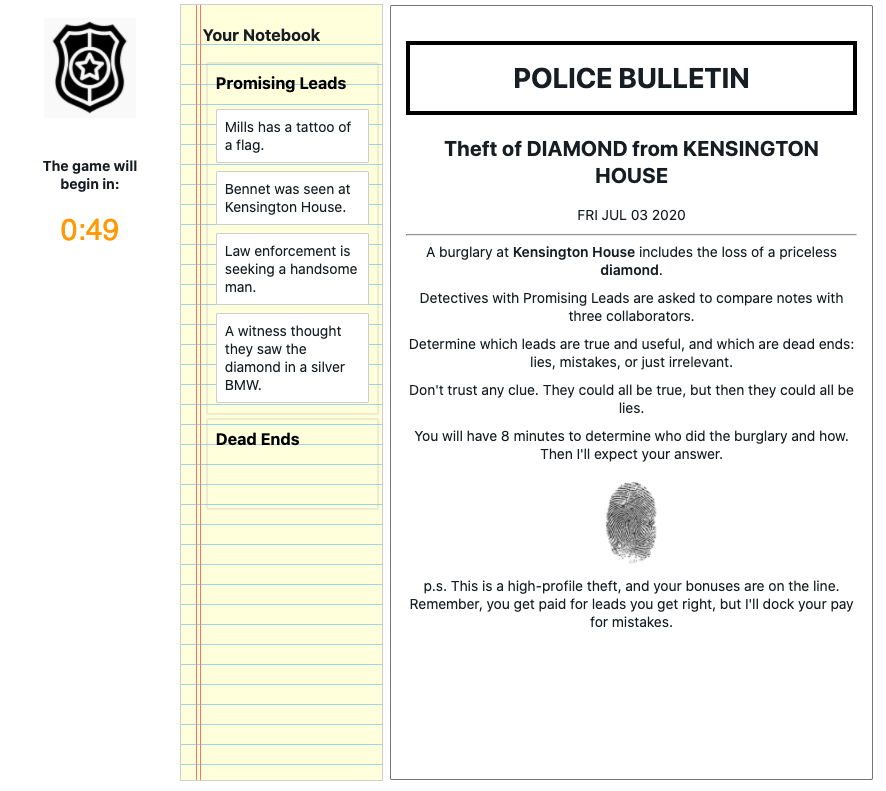
\includegraphics[width=0.7\columnwidth]{07_exposition.png}}
\caption{Exposition: Players were introduced to the case and reminded of their task when the game launched.}
\label{fig:exposition}
\end{figure}

\subsubsection{Playing the game: Exchanging clues}
When the game launched, the police bulletin was replaced with the promising leads sections of three collaborators’ notebooks, showing the participants a total of 16 unique clues at the start of the game. Individuals at corresponding positions in each social network were given clues that were as similar as possible while allowing for the intervention. These are shown for players in the treatment and control conditions in Figs. \ref{fig:interdependent_game} and \ref{fig:independent_game} respectively.

\begin{figure}[h!]
\centering
\fbox{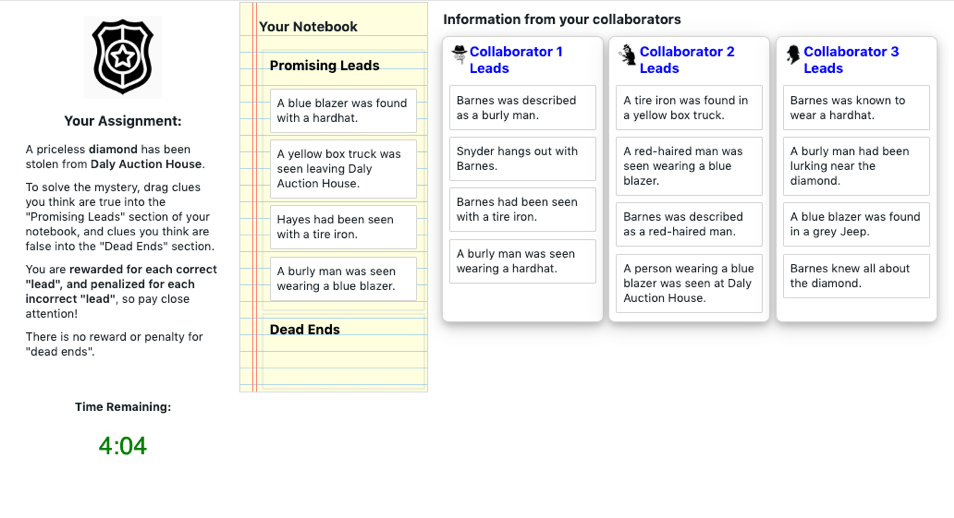
\includegraphics[width=1.0\columnwidth]{09_interdependent_game.png}}
\caption{Player interface with interdependent clue set}
\label{fig:interdependent_game}
\end{figure}

\begin{figure}[h!]
\centering
\fbox{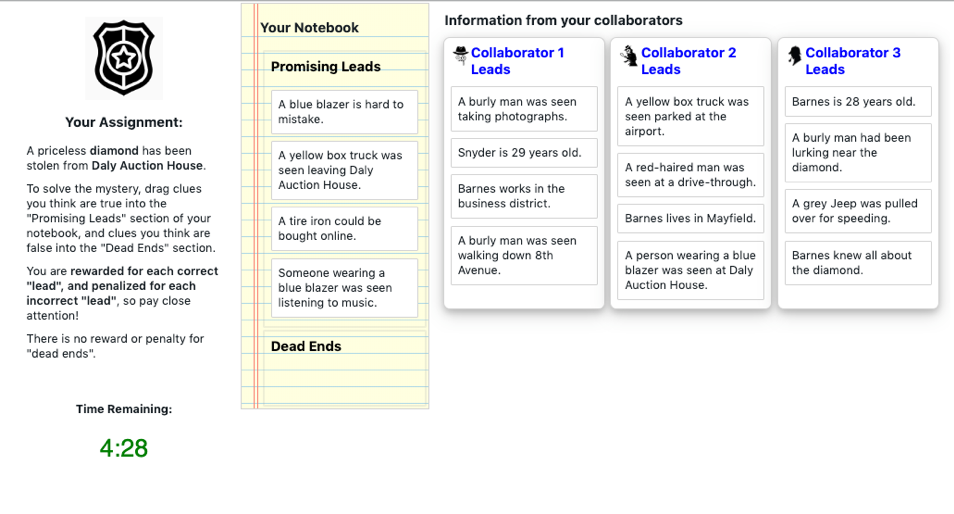
\includegraphics[width=1.0\columnwidth]{10_independent_game.png}}
\caption{Player interface with matching independent clue set}
\label{fig:independent_game}
\end{figure}

The game was played in real-time over 8 minutes. When a participant made any change to their promising leads, their neighbors immediately saw the change on their own screen. The starting clues of every individual were recorded, and every change to every player’s detective notebook was logged, such that the state of every player’s notebook can be reconstructed at each moment in the game. Participants were compensated \$1.00 for playing the game.

\subsubsection{Post-game survey: Making the case}

Following the game, participants were asked to assess (using a slider) how likely it was that certain individuals referenced in the game were the burglar, and how likely it was that they used various tools, vehicles, and disguises in the task. The first few of these questions are shown in Fig. \ref{fig:make_the_case}. Sliders were labeled from Extremely Unlikely to Extremely Likely, and responses were recorded on a scale from 0 to 100. Participants were also asked to assess their confidence in their solution, and to estimate the level of consensus among their team, as shown in Fig. \ref{fig:confidence}.

\begin{figure}[h!]
\centering
\fbox{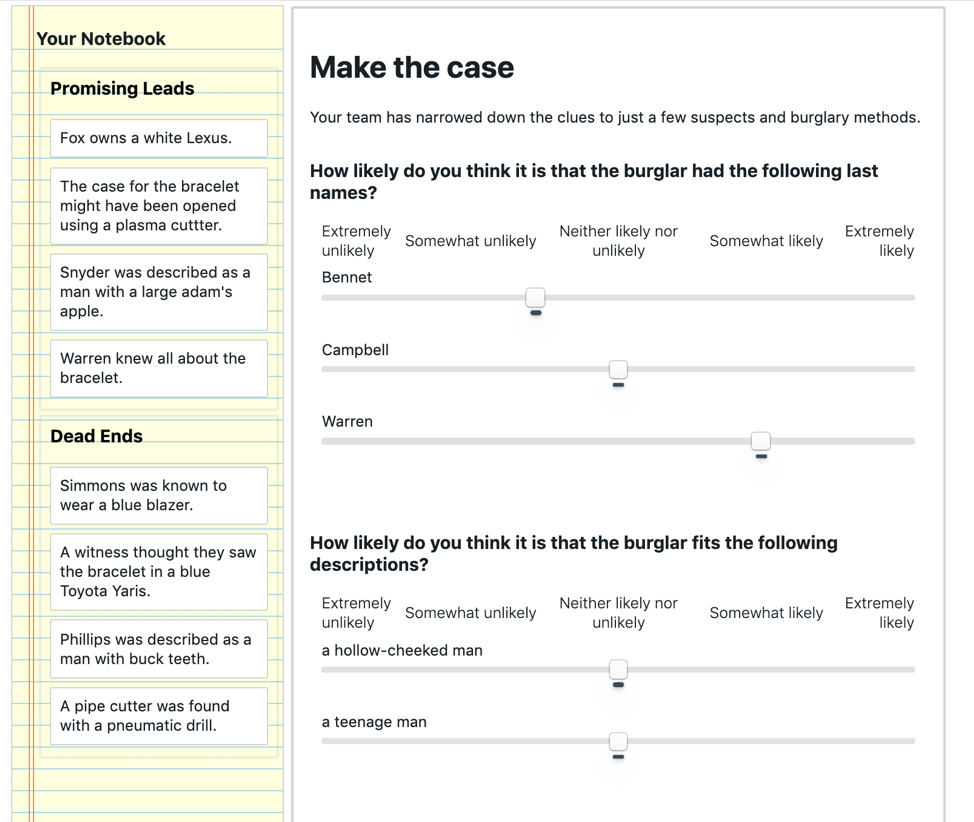
\includegraphics[width=0.8\columnwidth]{11_make_the_case.png}}
\caption{Post-game survey: Make the case for who committed the burglary}
\label{fig:make_the_case}
\end{figure}

\begin{figure}[h!]
\centering
\fbox{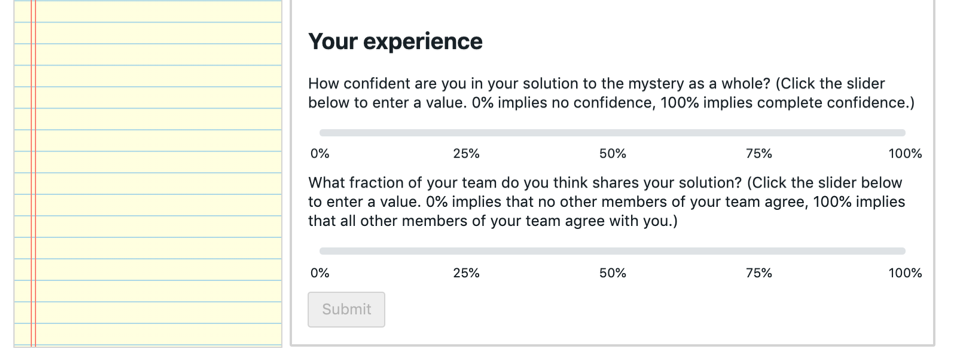
\includegraphics[width=0.8\columnwidth]{12_confidence.png}}
\caption{Post-game survey: Assess your confidence and estimate consensus}
\label{fig:confidence}
\end{figure}

After “Making the Case”, individuals were told that they were part of an experimental condition in which none of the clues were false, and they were rewarded \$0.10 for each clue in the promising leads section of their notebook, along with \$0.10 for each of the average number of clues their teammates had categorized as a promising lead. Participants were given a completion code to collect their bonuses, and an opportunity to report any problems with the game or describe their strategy. Many reported that they had enjoyed the game, and would like to play again.

% TODO: maybe add a screenshot of the thank-you screen?



\subsection{Experimental manipulation/stimulus}
\label{manipulation}
Clues were constructed from a bank of concepts (11 stolen objects, 11 crime scenes, 15 suspect names, 10 descriptions, 10 articles of clothing, 10 tools, and 10 vehicles) and a set of relationships (e.g. ``\{Name\} owns a \{vehicle\}'', ``A witness thought they saw \{stolen object\} in \{vehicle\}'') that formed a complete network between all concepts. This pool is sufficient to generate $11^2 * {15 \choose 3} * {10 \choose 2}^4 \approx 2.25\times10^{11}$ different mysteries.

\subsubsection{Constructing the bank of clue concepts}
The bank of concepts was constructed by starting with a pool of 403 candidate concepts including names, clothing, vehicles, etc. A pretest survey was conducted in which Amazon Mechanical Turk workers rated how likely each candidate concept was to have been used in a generic burglary. Individuals saw a subset of the concepts and were asked to give their gut reactions using a slider from Extremely Unlikely to Extremely Likely, as illustrated in Fig \ref{fig:clue_pretest}. In total, 139 participants rated each of the 403 candidate concepts between 20 and 30 times. Participants in the pretest were paid \$1.25 for a task which took each participant an average of about 4 minutes.

\begin{figure}[h!]
\centering
\fbox{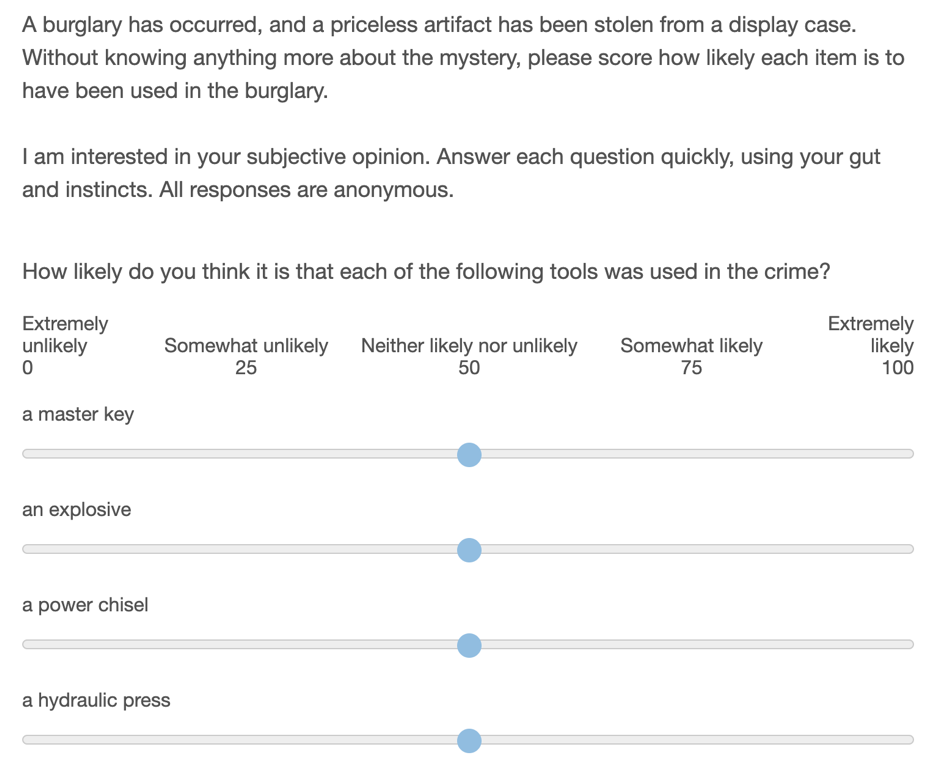
\includegraphics[width=0.7\columnwidth]{clue_pretest.png}}
\caption{Pretesting the perceived likelihood of each concept being involved in a crime}
\label{fig:clue_pretest}
\end{figure}

The pool of candidate names in the pretest represents the subset of the 200 most popular last names in the United States with a racial composition of between 50\% and 80\% ‘White’, as recorded in the 2000 US census. This selection is made to minimize the possibility of racial biases in the results. Additionally, names which are also common first names were excluded (e.g. “Stewart” or “Ross”) as were names which also serve as descriptors or adjectives in other clues (e.g. “Green”, “White”, or “Young”).

The remaining candidate concepts were written such that they would be as independent from one another as possible (e.g. I do not include both “a fat man” and “an overweight man” as these are synonymous, nor both “an old man” and “a man with grey hair” as these are perceived to go together.)

From the pretest results, I selected a subset of concepts that were perceived to be as likely as one another to be used in a burglary. (This helps to ensure that we do not see games in which all participants adopt “a set of lock picks” as a tool in the burglary, and reject “craft scissors”, just because lock picks are easier to imagine being used in a burglary.) The final selection was made by taking the subset of beliefs that minimized the difference in mean value of pretest survey responses when responses are normalized for each individual, and cross-checking against the means of the raw responses.

A similar pretest survey was conducted to select ‘spur’ clue concepts from a pool of candidates.



\newgeometry{margin=1cm} % modify this if you need even more space
\begin{landscape}

\begin{table}[]
\caption {Clue concept bank. Each element is perceived to be equally likely to have been involved in a burglary.} \label{tab:elements} 
\begin{tabular}{lllllll}
\textbf{CrimeScene}       & \textbf{StolenObject} & \textbf{Suspect} & \textbf{Clothing}        & \textbf{Appearance}   & \textbf{Tool}     & \textbf{Vehicle}          \\
the art museum            & the painting          & Collins          & a pair of overalls       & a long-haired man     & a hacksaw         & a yellow box truck        \\
the Pine Street Gallery   & the statue            & Hawkins          & a wool hat               & a pot-bellied man     & a serrated knife  & a blue Chevrolet Corvette \\
Kensington House          & the relic             & Mills            & a blue denim jacket      & a partially-bald man  & a set of hex keys & a green Mazda 3           \\
the Asper Casino          & the bracelet          & Cooper           & a tracksuit              & a grey-haired man     & a masonry drill   & a silver BMW              \\
the Danforth Hotel        & the antique           & Moore            & a pair of skinny-jeans   & a short man           & a circular saw    & a silver VW Jetta         \\
Knight Secure Storage     & the necklace          & Bennet           & a black scarf            & a well-groomed man    & a blowtorch       & a black Hummer            \\
the Daly Auction House    & the watch             & Mitchell         & a motorcycle helmet      & a man with sideburns  & an impact wrench  & a white Ford Fusion       \\
the Kentwood Mansion      & the diamond           & Stevens          & a black leather jacket   & a heavily-scarred man & a tire iron       & a blue Toyota Yaris       \\
the Dalhoff Estate        & the opal              & Wagner           & a pair of ripped jeans   & a blonde-haired man   & a pipe cutter     & a white Toyota Avalon     \\
the Darrowby Country Club & the crystal           & Edwards          & a blue long sleeve shirt & a handsome man        & a sledgehammer    & a blue Honda Fit          \\
DeRolfe Jewelers          & the jewel             & Rice             &                          &                       &                   &                           \\
                          &                       & Roberts          &                          &                       &                   &                           \\
                          &                       & Daniels          &                          &                       &                   &                           \\
                          &                       & Warren           &                          &                       &                   &                           \\
                          &                       & Sullivan         &                          &                       &                   &                          
\end{tabular}
\end{table}
\end{landscape}
\restoregeometry

% interdependent diffusion edges
\newgeometry{margin=1cm} % modify this if you need even more space
\begin{landscape}
\begin{table}[]
\caption {Interdependent clue connections together create a complete knowledge graph.} \label{tab:inter_edges} 
\begin{tabular}{ll}
\{StolenObject\_1\}   was kept in a case at \{CrimeScene\_1\} & \{Suspect\_2\} had been seen with   \{Tool\_2\} \\
\{Suspect\_1\}   was seen at \{CrimeScene\_1\} & \{Suspect\_2\} owns \{Vehicle\_1\} \\
\{Suspect\_2\}   was seen at \{CrimeScene\_1\} & \{Suspect\_2\} owns \{Vehicle\_2\} \\
\{Suspect\_3\}   was seen at \{CrimeScene\_1\} & \{Suspect\_3\} was known to wear   \{Clothing\_1\} \\
A person   wearing \{Clothing\_1\} was seen at \{CrimeScene\_1\} & \{Suspect\_3\} was known to wear   \{Clothing\_2\} \\
A person   wearing \{Clothing\_2\} was seen at \{CrimeScene\_1\} & \{Suspect\_3\} was described as   \{Appearance\_1\} \\
\{Appearance\_1\}   was seen at \{CrimeScene\_1\} & \{Suspect\_3\} was described as   \{Appearance\_2\} \\
\{Appearance\_2\}   was seen at \{CrimeScene\_1\} & \{Suspect\_3\} had been seen with   \{Tool\_1\} \\
Evidence   at \{CrimeScene\_1\} indicates the use of \{Tool\_1\} & \{Suspect\_3\} had been seen with   \{Tool\_2\} \\
Evidence   at \{CrimeScene\_1\} indicates the use of \{Tool\_2\} & \{Suspect\_3\} owns \{Vehicle\_1\} \\
\{Vehicle\_1\}   was seen leaving \{CrimeScene\_1\} & \{Suspect\_3\} owns \{Vehicle\_2\} \\
\{Vehicle\_2\}   was seen leaving \{CrimeScene\_1\} & \{Clothing\_1\} was found with   \{Clothing\_2\} \\
\{Suspect\_1\}   knew all about \{StolenObject\_1\} & \{Appearance\_1\} was seen wearing   \{Clothing\_1\} \\
\{Suspect\_2\}   knew all about \{StolenObject\_1\} & \{Appearance\_2\} was seen wearing   \{Clothing\_1\} \\
\{Suspect\_3\}   knew all about \{StolenObject\_1\} & \{Clothing\_1\} was found with   \{Tool\_1\} \\
A person   wearing \{Clothing\_1\} had been seen lurking near \{StolenObject\_1\} & \{Clothing\_1\} was found with   \{Tool\_2\} \\
A person   wearing \{Clothing\_2\} had been seen lurking near \{StolenObject\_1\} & \{Clothing\_1\} was found in   \{Vehicle\_1\} \\
\{Appearance\_1\}   had been lurking near \{StolenObject\_1\} & \{Clothing\_1\} was found in   \{Vehicle\_2\} \\
\{Appearance\_2\}   had been lurking near \{StolenObject\_1\} & \{Appearance\_1\} was seen wearing   \{Clothing\_2\} \\
The case   for \{StolenObject\_1\} might have been opened using \{Tool\_1\} & \{Appearance\_2\} was seen wearing   \{Clothing\_2\} \\
The case   for \{StolenObject\_1\} might have been opened using \{Tool\_2\} & \{Clothing\_2\} was found with   \{Tool\_1\} \\
A   witness thought they saw \{StolenObject\_1\} in \{Vehicle\_1\} & \{Clothing\_2\} was found with   \{Tool\_2\} \\
A   witness thought they saw \{StolenObject\_1\} in \{Vehicle\_2\} & \{Clothing\_2\} was found in   \{Vehicle\_1\} \\
\{Suspect\_2\}   hangs out with \{Suspect\_1\} & \{Clothing\_2\} was found in   \{Vehicle\_2\} \\
\{Suspect\_1\}   hangs out with \{Suspect\_3\} & \{Appearance\_2\} was seen with   \{Appearance\_1\} \\
\{Suspect\_1\}   was known to wear \{Clothing\_1\} & \{Appearance\_1\} was seen with   \{Tool\_1\} \\
\{Suspect\_1\}   was known to wear \{Clothing\_2\} & \{Appearance\_1\} was seen with   \{Tool\_2\} \\
\{Suspect\_1\}   was described as \{Appearance\_1\} & \{Appearance\_1\} was seen driving   \{Vehicle\_1\} \\
\{Suspect\_1\}   was described as \{Appearance\_2\} & \{Appearance\_1\} was seen driving   \{Vehicle\_2\} \\
\{Suspect\_1\}   had been seen with \{Tool\_1\} & \{Appearance\_2\} was seen with   \{Tool\_1\} \\
\{Suspect\_1\}   had been seen with \{Tool\_2\} & \{Appearance\_2\} was seen with   \{Tool\_2\} \\
\{Suspect\_1\}   owns \{Vehicle\_1\} & \{Appearance\_2\} was seen driving   \{Vehicle\_1\} \\
\{Suspect\_1\}   owns \{Vehicle\_2\} & \{Appearance\_2\} was seen driving   \{Vehicle\_2\} \\
\{Suspect\_3\}   hangs out with \{Suspect\_2\} & \{Tool\_1\} was found with \{Tool\_2\} \\
\{Suspect\_2\}   was known to wear \{Clothing\_1\} & \{Tool\_1\} was found in   \{Vehicle\_1\} \\
\{Suspect\_2\}   was known to wear \{Clothing\_2\} & \{Tool\_1\} was found in   \{Vehicle\_2\} \\
\{Suspect\_2\}   was described as \{Appearance\_1\} & \{Tool\_2\} was found in   \{Vehicle\_1\} \\
\{Suspect\_2\}   was described as \{Appearance\_2\} & \{Tool\_2\} was found in   \{Vehicle\_2\} \\
\{Suspect\_2\}   had been seen with \{Tool\_1\} & \{Vehicle\_2\} was found near   \{Vehicle\_1\}
\end{tabular}
\end{table}

\end{landscape}
\restoregeometry


% filler clues
\newgeometry{margin=1cm} % modify this if you need even more space
\begin{landscape}

\begin{table}[]
\caption {Filler element bank. Each element equally influences the perception that an associated concept was involved in a burglary.} \label{tab:filler} 
\begin{tabular}{lllll}
\textbf{suspectAge} & \textbf{suspectConviction} & \textbf{suspectMeans}                          & \textbf{suspectMotive}                    & \textbf{suspectTattoo} \\
33 years old        & drug possession            & was trained as a welder                        & has paid hush-money to a former lover     & a compass              \\
37 years old        & fraud                      & installs security systems                      & has family connections to organized crime & a bear                 \\
in their early 30's & drug distribution          & was trained as a goldsmith                     & is deep in payday-loan debt               & a heart                \\
in their mid 20's   & running a Ponzi scam       & has worked as an automotive repossession agent & has an expensive drug habit               & a flower               \\
in their late 20's  & embezzlement               & has worked as a security guard                 & has a gambling addiction                  & a clock                \\
in their late 30's  & identity theft             & worked at a pawn shop                          & wrote a revolutionary manifesto           & a star                 \\
in their early 20's & perjury                    & has worked as an armored car driver            & had been involved in gang activity        & a dog                  \\
29 years old        & shoplifting                & has worked for an import/export company        & has large gambling debts                  & a crown                \\
36 years old        & arson                      & worked for an alarm company                    & has a heroin addiction                    & a flag                
\end{tabular}
\end{table}



\begin{table}[]
\begin{tabular}{lllll}
\textbf{appearanceInjury} & \textbf{appearanceRemoved} & \textbf{appearanceReported}   & \textbf{appearanceStreet} & \textbf{appearanceWanted}                         \\
a broken arm              & a museum                   & waiting in a dark alley       & Maple Avenue              & Law enforcement is seeking                        \\
a fractured kneecap       & a public library           & shouting at 11pm              & Lincoln Boulevard         & Officers are asking questions about               \\
a concussion              & a bar                      & sitting in a tree             & Chestnut Street           & Private security companies have been warned to... \\
a fractured rib           & a restaurant               & painting graffiti             & Church Street             & Airport security has been asked to look out for   \\
minor burns               & a residence                & vandalizing a vending machine & Hill Street               & Police are interviewing witnesses about           \\
a drug overdose           & a party                    & carrying a large bag          & Ninth Avenue              & Information is wanted about                      
\end{tabular}
\end{table}

\begin{table}[]
\begin{tabular}{lllll}
\textbf{carBehavior}                     & \textbf{carBuy}          & \textbf{carDamage}    & \textbf{carEnterprise} & \textbf{carTicketed}       \\
driving after midnight                   & in a wholesale auction   & a broken headlight    & a club                 & an expired registration    \\
with someone sleeping in the   back seat & at a police auction      & a broken grill        & a massage parlor       & parking in a loading zone  \\
with darkly tinted windows               & from a classified ad     & damaged suspension    & a strip mall           & driving without headlights \\
parked in a lot for multiple   nights    & at an estate sale        & a missing wing mirror & a laundromat           & a broken tail light        \\
taking the back streets                  & from a used-car salesmen & the airbags deployed  & a delicatessen         & illegal parking            \\
with its hood up on the   roadside       & from a junk-yard         & a broken axle         & a hotel                & running a stop sign       
\end{tabular}
\end{table}

\begin{table}[]
\begin{tabular}{lllll}
\textbf{clothingActivity}             & \textbf{clothingDamage} & \textbf{clothingDiscoverer}                  & \textbf{clothingFootage} & \textbf{clothingWith}                  \\
pacing back and forth                 & cut into pieces         & a gym owner emptying abandoned lockers       & at a bus stop            & a list of tools                        \\
entering a machine room               & with tire marks on it   & a dockworker moving shipping pallets         & in the woods             & a home-made electronic device          \\
pulling an object out of a   gutter   & with frayed edges       & a store worker breaking down cardboard boxes & in the park              & a pair of rubber gloves                \\
looking through binoculars at   night & burned in a fire        & a journalist uncovering a story              & at a campsite            & an inter-city train schedule           \\
getting into a taxi                   & discolored with bleach  & a postal worker emptying a mailbox           & on a bridge              & the stub of a bus ticket               \\
climbing on a bridge                  & caked in mud            & theater staff cleaning up after a movie      & on the golf course       & an envelope containing GPS coordinates
\end{tabular}
\end{table}

\begin{table}[]
\begin{tabular}{lllll}
\textbf{toolDamage}                         & \textbf{toolFound}    & \textbf{toolUse}               & \textbf{toolWith}                  & \textbf{toolrandom}                            \\
showing signs of misuse                     & buried in debris      & access maintenance crawlspaces & with a pair of work gloves         & could be used by one person                    \\
with minor damage                           & in an abandoned house & open an upper-story window     & with safety features removed       & has been used in prior burglaries \\
with burn marks                             & in a trash compactor  & bypass an alarm system         & that had been painted black        & could be concealed in a backpack               \\
disassembled into pieces & in a garage           & deactivate a motion sensor     & with gunpowder residue             & leaves distinctive marks if used carelessly    \\
covered in sawdust  & in a creek            & disassemble an alarm panel     & wrapped in newspaper               & is often used by thieves                       \\
\begin{minipage}[t]{0.15\columnwidth}that had been damaged falling from a height\end{minipage}                    & beside a road         & circumvent a lock              & wrapped in tape to make it quieter & \begin{minipage}[t]{0.25\columnwidth}was shown in news coverage of another burglary  \end{minipage}      
\end{tabular}
\end{table}

\end{landscape}
\restoregeometry


\newgeometry{margin=1cm} % modify this if you need even more space
\begin{landscape}
 
\begin{table}[]
\caption {Independent clue connections break relationships between analysis clues} \label{tab:indep_edges} 
\begin{tabular}{ll}
\{StolenObject\_1\}   was kept in a case at \{CrimeScene\_1\} & A constable noticed   \{Appearance\_1\} on \{appearanceStreet\_1\} \\
\{Suspect\_1\}   was seen at \{CrimeScene\_1\} & A constable noticed   \{Appearance\_2\} on \{appearanceStreet\_2\} \\
\{Susect\_2\}   was seen at \{CrimeScene\_1\} & \{Tool\_1\} was found \{toolWith\_1\} \\
\{Suspect\_3\}   was seen at \{CrimeScene\_1\} & \{Tool\_2\} was found \{toolWith\_2\} \\
A person   wearing \{Clothing\_1\} was seen at \{CrimeScene\_1\} & \{Vehicle\_1\} was recently   purchased \{carBuy\_1\} \\
A person   wearing \{Clothing\_2\} was seen at \{CrimeScene\_1\} & \{Vehicle\_2\} was recently   purchased \{carBuy\_2\} \\
\{Appearance\_1\}   was seen at \{CrimeScene\_1\} & \{Suspect\_1\} is \{suspectAge\_1\} \\
\{Appearance\_2\}   was seen at \{CrimeScene\_1\} & \{Suspect\_2\} is \{suspectAge\_2\} \\
Evidence   at \{CrimeScene\_1\} indicates the use of \{Tool\_1\} & \{Suspect\_3\} is \{suspectAge\_3\} \\
Evidence   at \{CrimeScene\_1\} indicates the use of \{Tool\_2\} & \{Clothing\_1\} was discovered by   \{clothingDiscoverer\_1\} \\
\{Vehicle\_1\}   was seen leaving \{CrimeScene\_1\} & \{Clothing\_2\} was discovered by   \{clothingDiscoverer\_2\} \\
\{Vehicle\_2\}   was seen leaving \{CrimeScene\_1\} & \{Appearance\_1\} was reported   \{appearanceReported\_1\} \\
\{Suspect\_1\}   knew all about \{StolenObject\_1\} & \{Appearance\_2\} was reported   \{appearanceReported\_2\} \\
\{Suspect\_2\}   knew all about \{StolenObject\_1\} & \{Tool\_1\} could be used to   \{toolUse\_1\} \\
\{Suspect\_3\}   knew all about \{StolenObject\_1\} & \{Tool\_2\} could be used to   \{toolUse\_2\} \\
A person   wearing \{Clothing\_1\} had been seen lurking near \{StolenObject\_1\} & \{Vehicle\_1\} was ticketed for   \{carTicketed\_1\} \\
A person   wearing \{Clothing\_2\} had been seen lurking near \{StolenObject\_1\} & \{Vehicle\_2\} was ticketed for   \{carTicketed\_2\} \\
\{Appearance\_1\}   had been lurking near \{StolenObject\_1\} & \{Suspect\_1\} \{suspectMeans\_1\} \\
\{Appearance\_2\}   had been lurking near \{StolenObject\_1\} & \{Suspect\_2\} \{suspectMeans\_2\} \\
The case   for \{StolenObject\_1\} might have been opened using \{Tool\_1\} & \{Suspect\_3\} \{suspectMeans\_3\} \\
The case   for \{StolenObject\_1\} might have been opened using \{Tool\_2\} & \{Clothing\_1\} was found with   \{clothingWith\_1\} \\
A   witness thought they saw \{StolenObject\_1\} in \{Vehicle\_1\} & \{Clothing\_2\} was found with   \{clothingWith\_2\} \\
A   witness thought they saw \{StolenObject\_1\} in \{Vehicle\_2\} & \{Appearance\_1\} was treated for   \{appearanceInjury\_1\} \\
\{Suspect\_1\}   has a tattoo of \{suspectTattoo\_1\} & \{Appearance\_2\} was treated for   \{appearanceInjury\_2\} \\
\{Suspect\_2\}   has a tattoo of \{suspectTattoo\_2\} & An FBI agent found \{Tool\_1\}   \{toolFound\_1\} \\
\{Suspect\_3\}   has a tattoo of \{suspectTattoo\_3\} & An FBI agent found \{Tool\_2\}   \{toolFound\_2\} \\
A   policeman saw someone in \{Clothing\_1\} \{clothingActivity\_1\} & An officer identified   \{Vehicle\_1\} at \{carEnterprise\_1\} \\
A   policeman saw someone in \{Clothing\_2\} \{clothingActivity\_2\} & An officer identified   \{Vehicle\_2\} at \{carEnterprise\_2\} \\
\{appearanceWanted\_1\}   \{Appearance\_1\} & \{Suspect\_1\} has a prior   conviction for \{suspectConviction\_1\} \\
\{appearanceWanted\_2\}   \{Appearance\_2\} & \{Suspect\_2\} has a prior   conviction for \{suspectConviction\_2\} \\
\{Tool\_1\}   \{toolrandom\_1\} & \{Suspect\_3\} has a prior   conviction for \{suspectConviction\_3\} \\
\{Tool\_2\}   \{toolrandom\_2\} & Forensics identified   \{Clothing\_1\} \{clothingDamage\_1\} \\
\{Vehicle\_1\}   was reported \{carBehavior\_1\} & Forensics identified   \{Clothing\_2\} \{clothingDamage\_2\} \\
\{Vehicle\_2\}   was reported \{carBehavior\_2\} & \{Appearance\_1\} was forcibly   removed from \{appearanceRemoved\_1\} \\
\{Suspect\_1\}   \{suspectMotive\_1\} & \{Appearance\_2\} was forcibly   removed from \{appearanceRemoved\_2\} \\
\{Suspect\_2\}   \{suspectMotive\_2\} & A forensics report contained   \{Tool\_1\} \{toolDamage\_1\} \\
\{Suspect\_3\}   \{suspectMotive\_3\} & A forensics report contained   \{Tool\_2\} \{toolDamage\_2\} \\
Someone   wearing \{Clothing\_1\} was seen on security footage \{clothingFootage\_1\} & \{Vehicle\_1\} was found with   \{carDamage\_1\} \\
Someone   wearing \{Clothing\_2\} was seen on security footage \{clothingFootage\_2\} & \{Vehicle\_2\} was found with   \{carDamage\_2\}
\end{tabular}
\end{table}

\end{landscape}
\restoregeometry

\subsubsection{Assembling sets of clues for use in games}
This experiment manipulates the structure of clues within the detective game, to create an ``interdependent'' condition in which the clues interact strongly with each other, and an ``independent'' condition that limits those interactions while preserving as much similarity with the treatment condition as possible. 

Clues were constructed in three waves. The first wave was identical for both conditions, and is illustrated in Fig. \ref{fig:spokes}. Clues were created that link ‘hub’ concepts (including a crime scene and a stolen object) to ‘rim’ concepts (including three suspects, two articles of clothing, two physical descriptions, two tools, and two vehicles). For example “\textbf{Hayes} was seen at the \textbf{Daly Auction House}” or “The case for the \textbf{diamond} might have been opened using a \textbf{circular saw}”. “Spoke” clues were independent of one another, as they could only interact via association with the crime scene and stolen object – items that were known in advance to be relevant to the mystery. There were 11 rim concepts and 2 hub concepts, and so 22 spoke clues.

\begin{figure}[h!]
\centering
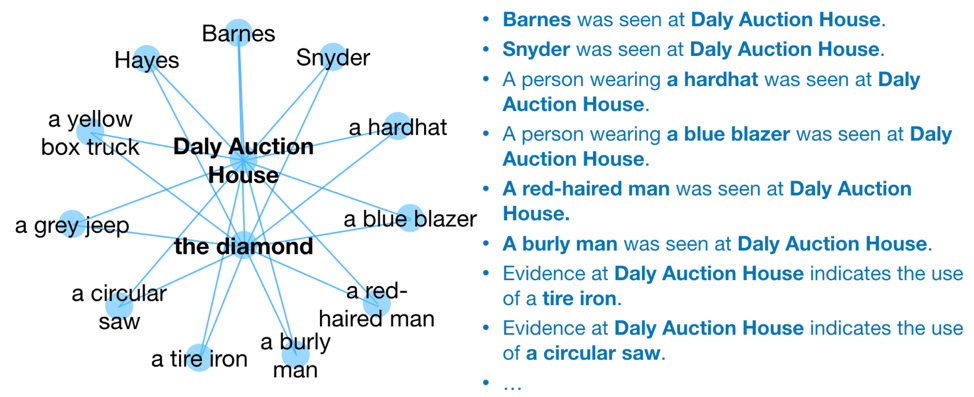
\includegraphics[width=0.7\columnwidth]{Spoke Clues.png}
\caption{Wave 1 of clue generation created ``spoke'' or analysis clues used in both treatment and control games. ``Spoke'' clues connected rim concepts to hub concepts.}
\label{fig:spokes}
\end{figure}

In the interdependent condition, the second wave of clue construction created ``cross-link'' clues, which connected each of the spoke clues to one another (e.g. ``\textbf{Hayes} owns a \textbf{circular saw}''). These cross-link clues create interdependence between the spoke clues, and allow for clues to logically support one another (e.g. if I believe that ``A burly man was seen at the Daly Auction House'' and that ``Barnes is a burly man'', then I am more receptive to the idea that ``Barnes was seen at the Daly Auction House''). A cross-link clue connected each of the 11 rim concepts to the other rim concepts, for a total of 55 unique cross-link clues, as shown in Fig. \ref{fig:crosslinks}.

\begin{figure}[h!]
\centering
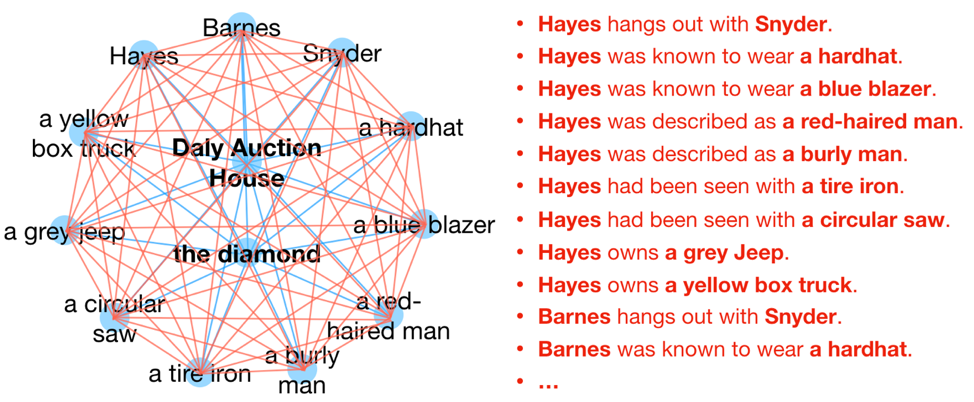
\includegraphics[width=0.7\columnwidth]{crosslink clues.png}
\caption{Wave 2 of clue generation created ``cross-link'' clues for the interdependent condition. Cross-link clues connect rim concepts to one another.}
\label{fig:crosslinks}
\end{figure}

In the independent condition, the second wave of clue construction created “spur” clues that connected to the rim concepts, but did not connect to other clues (Fig \ref{fig:spurs}). There were the same number of spur clues in the independent condition as cross-link clues in the interdependent condition: 55. By connecting to the rim concepts (rather than being disconnected altogether) these clues help separate the effect of interdependence manifest as logical relationships between clues from the effect of the frequency of each rim concept in the set of clues. The content of the spur clues was selected in pretest to have a uniform impact on participants judgement of the rim element to which they connect. 

\begin{figure}[h!]
\centering
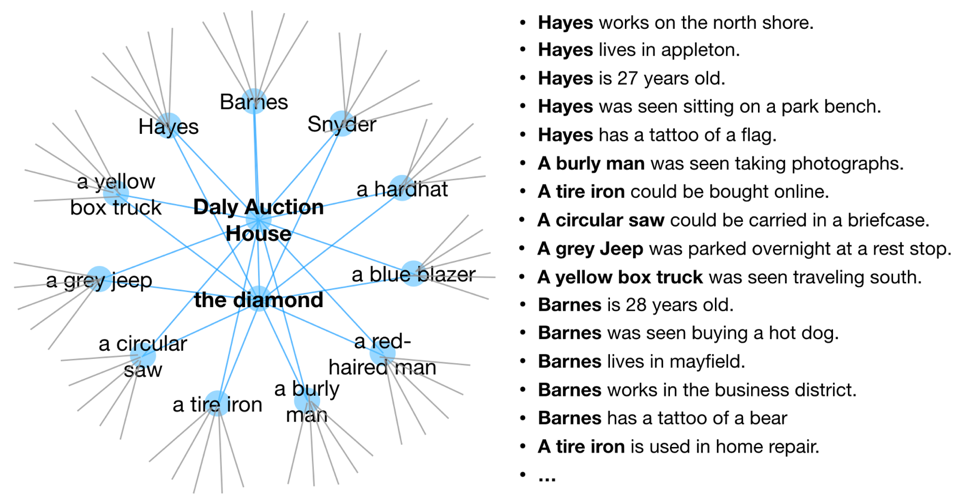
\includegraphics[width=0.7\columnwidth]{Spur Clues.png}
\caption{Wave 2 of clue generation created ``spur'' clues for the independent condition. Spur clues filled the place of cross-link clues without creating links between rim concepts. Spur clues still allowing for multiple exposures to rim concepts.}
\label{fig:spurs}
\end{figure}

The first and second waves of clue construction created 77 unique clues. As there were 20 individuals in each treatment within each game, 80 clues were needed to give each individual 4 starting clues. The third wave of clue construction filled the 3 remaining spaces with the clue connecting the crime scene to the stolen object (e.g. The \textbf{diamond} was stolen from the \textbf{Daly Auction House}.) This was redundant information, as all participants were told this at the start of the game. 


\subsection{Data collection and measurements}
\label{data_collection}
Sufficient data was collected to replicate the state of the game at any point during game play, and to observe every action taken by every player.

\subsubsection{Recording player actions}
In addition to the social network structure and the initial assignment of clues to positions within the social network, the following information was recorded:
\begin{enumerate}
    \item Each drag event that resulted in a change in a player’s notebook (i.e. addition of a clue to a notebook section OR change of order within a notebook section) was logged. Logging information includes the ID of the clue being dropped, the source for the drag event (i.e. the exposing player or notebook the belief came from), the destination for the drag event (i.e. the notebook the clue is being dragged into), the position within the destination notebook that the clue moved into (i.e. its index in the list) and the time at which the drop event occurred.
    \item The final state of all detectives' notebooks was recorded. Together with the initial state, this provides a check that all events were logged properly.
    \item Each individual provided a self-report of the degree to which they believed each of the 11 “rim” concepts to be connected to the crime, collected using an empty slider from “Extremely Unlikely” to “Extremely Likely”. Slider positions were captured as an integer value between 0 and 100.
    \item Individuals reported their confidence in their solution on a scale from 0 to 100 using a blank slider. 
    \item Individuals reported the fraction of their team they thought shared their solution on a scale from 0 to 100 percent, using a blank slider.
    \item Individuals reported their Age, Education, Gender, and feedback on the game.
\end{enumerate}

\subsubsection{Choice of summary statistics}

The \textbf{similarity between individuals' self-reported beliefs} was measured using Pearson's correlation coefficient. 
As others have identified, \cite{goldberg2018beyond} correlation is a natural measure when we have a fixed number of continuous measures of each subject. It is readily interpretable, and the fixed range (-1,1) maps to intuitive understandings of similarity and difference.
	
The \textbf{similarity between individuals' behavior} was measured using the Phi coefficient. This measure corresponds to Pearson correlation when values are binary, and has the same interpretable (-1,1) range. 
The phi coefficient is appropriate for a universe with a finite number of beliefs, but would be less appropriate as the number of adopted beliefs becomes a very small fraction of the total number of possible beliefs. 

The \textbf{alignment of the population along a ``left-right axis''} was measured as the percent of variance present in the first principal component, using singular value decomposition.
This measure corresponds to the notion of “constraint” articulated by Dimaggio et al. (\cite{dimaggio1996have}). In their paper they describe Chronbach’s alpha and the PCA measure both providing similar measures of constraint. I have chosen the PCA measure here as more interpretable, as it maps better to our intuitive understanding of a political spectrum.

The \textbf{within-camp and across-camp similarities} were measured as the 5\textsuperscript{th} and 95\textsuperscript{th} percentile similarities according to the similarity measures above. 
There are a number of different measures in the literature that try to capture the notion that with polarization, the most similar individuals become more self-similar, and the least similar individuals move further away from one another. 
The fact that no single measure has emerged as the leader hints at problems with each.
When the identities of camps are already known the difference of means between groups can be used (\cite{becker2019wisdom},\cite{dimaggio1996have}). 
Variance (see \cite{baldassarri2007dynamics},\cite{dimaggio1996have}) captures heterogeneity between individuals, but not clustering into camps. 
Kurtosis (\cite{baldassarri2007dynamics},\cite{dimaggio1996have}) is predicated on a bimodal distribution. 
The “gap” statistic (\cite{goldberg2018beyond}) is one of dozens of ways of assessing the quality of a machine learning clustering algorithm.

As I do not need to identify the groups themselves, or compare to external datasets, it is sufficient to merely report what each of these other measures is trying to approximate: the similarity that is found within groups, and that which is found across groups. As I am only interested in the relative differences between conditions (or changes over time) then I can arbitrarily designate a threshold for which comparisons will be considered ``within-group'' or ``across groups''. This provides a much more intuitive demonstration of increasing polarization than the measures found in above literature.

The closer the chosen thresholds are to the tails of the distribution, the more conservative the claim that the comparisons beyond this threshold are appropriately ``within'' or ``across'' groups. At the same time, we need enough samples included in the set to minimize noise due to the finite number of comparisons. In this 20-participant social network, the 95\textsuperscript{th} and 5\textsuperscript{th} percentiles correspond to 10 comparisons between individuals. The sensitivity of results to the choice of these thresholds is explored in section \ref{section:thresholds} of this supplement.

For behavioral measures of within and across-camp similarity (i.e. those based upon clues identified as promising leads at the end of the game) these percentiles are sensitive not only to interdependence and network structure, but also to the average level of diffusion of clues. As the average level of diffusion can vary between games due to differences in players' baseline activity levels, this additional source of noise increases the sample size we would require to see an effect. To compensate for this noise, we can compare the percentiles to what would be expected due to chance, given the same extent of diffusion. To calculate the effect of interdependence and network structure, I first remove some of the noise by subtracting the 5\textsuperscript{th} and 95\textsuperscript{th} percentile values from a shuffled data-set that keeps the number of adopters of each clue and the number of clues adopted by each participant fixed. This makes for an apples-to-apples comparison of the effects of interdependence or network structure. This correction was designed in simulation and included in the preregistration for the experiment.

\subsubsection{Handling missing data}

As the game was played in real-time, the effect of a participant ‘dropping out’ during game-play was equivalent to them holding their beliefs fixed for the remainder of the game. As it is impossible to distinguish these two behaviors, I identified a drop-out as any player failing to submit the post-game survey. 

When an individual failed to complete the post-game survey, aggregate results for their condition were calculated based upon the remaining players. Aggregate results for the paired comparison conditions were calculated as the average of all same-sized subsets of players in each comparison condition.

\subsection{Preregistration}
\label{prereg}

The preregistration for the experiment included all the code necessary to run and analyze the experiment presented in this paper, such that a direct replication can be conducted from the preregistered materials. The preregistration is available at \href{https://osf.io/239ns}{https://osf.io/239ns}. In addition to the analyses presented in this paper, the preregistration also included a secondary analysis of mediating and moderating effects of interdependent diffusion that will be reported in a second paper. 

The experiment differed from the preregistered procedure in three minor ways: expanding the recruitment pool, correcting a coding mistake, and formalizing an analysis that was preregistered with only a text description.

\begin{enumerate}
    \item The preregistered strategy of recruiting individuals with a “sign-up” HIT immediately prior to each game did not scale well to multiple games per day. Instead, I drew on a pool of Mechanical Turk workers from the US and Canada that had been recruited for a previous experiment. As the locations of the panelists were not recorded, this required me to relax the preregistered participant qualifications to include Canadian workers. I felt that this addition would not significantly influence the likelihood of success of the experiment or it’s generalizability. The phenomenon under study is not expected to behave differently in different populations, and the study does not require any special outside knowledge.
    
    \item The analysis code for comparing end-of-game measures was designed originally to account for dropouts in a (treatment/control) game by averaging over same-sized subsets of the matching (control/treatment) game. However, the code as preregistered did not account for the fact that comparisons should be made between four experimental conditions instead of two. The code was revised to make the correct comparisons.
    
    \item While the interaction analysis was included in the text of the preregistration, the code for computing it was mistakenly omitted. This additional code is included in the experiment repository.

\end{enumerate}

\subsection{Outcomes}
\label{outcomes}

\subsubsection{Participants' experience}

Participants were Amazon Mechanical Turk workers who lived in the US or Canada and were over 18 years of age. Workers must have completed at least 100 HITs and have a 90\% or better approval rating. Recruitment and compensation were handled using TurkPrime (\url{www.cloudresearch.com}).

For blocks 0-2, recruitment took place in the hour preceding a game launch via a timed “sign-up” HIT. This recruitment strategy had been shown to be effective during pilots, but did not scale well when multiple blocks were run during the same day. For blocks 3-29, recruitment took advantage of a panel of workers who had previously indicated willingness to be notified of upcoming games. This panel was expanded through ongoing paid and unpaid recruitment HITs during the period the experiments were run. Panel members were notified via email at the beginning of each day when experiments would take place, and again 10 minutes prior to the launch of a game. At the scheduled game time, HITs were made available to any worker meeting the qualifications, whether they were in the original panel or not. 

Participants were compensated \$0.10 for accepting the game HIT, in addition to \$1 for training, \$1 for playing the game, and up to \$2 in bonuses. Participants who trained but were unable to play were eligible to attempt to play again. Those who completed training and entered the game were blocked from participating in future games via an exclusion qualification.

\begin{figure}[H]
\centering
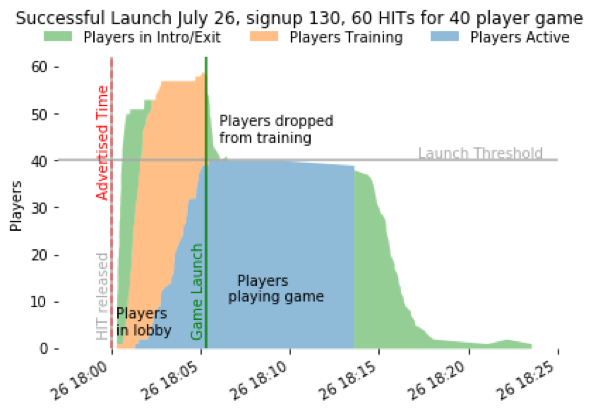
\includegraphics[width=0.6\columnwidth]{recruitment.png}
\caption{Players active by stage and time. (Data from pilot test.)}
\label{fig:recruitment}
\end{figure}

The game took about 20 minutes to play, including training, waiting room, and follow-up. The average payout was approximately \$4.00, for an hourly rate of approximately \$12.00/hr. Participants who trained but were unable to play spent about 5 minutes in the platform before they were bumped. They earned \$1.10, for an approximate hourly rate of \$13.20.  Fig. \ref{fig:recruitment} shows the number of participants active in different parts of the game at different times for a 2-condition pilot test. There were necessarily some individuals who were dropped from training when the game launched, as the number of individuals who would showed up for a game was unpredictable.



\subsubsection{Detailed Results}
Over eight minutes of gameplay, participants on average made 28.4 classifications and adopted 16.2 clues as promising leads. 
Despite the symmetry of the setup, and the fact that there was by design no solution to the mystery, participants came to strongly-held beliefs about which suspect was guilty and how they performed the crime. On average, participants felt that the most likely suspect was almost 50\% more likely to be involved in the crime than the least likely suspect, and over half of participants reported confidence in at least one part of their solution of 95\% or greater. Table \ref{Tab:effect_summary} reports the effect sizes for all comparisons made in the experiment.

% \begin{table}[H]
% \centering
% \caption{Effect and Interaction Summary}
% \label{Tab:effect_summary}
% \begin{tabular}{llcccc}
% \hline
%  &
%   \multicolumn{1}{l|}{} &
%   \multicolumn{3}{c|}{\textbf{Effect over baseline condition}} &
%   \multirow{4}{*}{\begin{tabular}[c]{@{}c@{}}Interaction of\\ Interdep Clues\\ and Polarizing\\ Network\end{tabular}} \\
%  &
%   \multicolumn{1}{l|}{} &
%   \begin{tabular}[c]{@{}c@{}}Interdep\\ Clues Alone\end{tabular} &
%   \begin{tabular}[c]{@{}c@{}}Polarizing\\ Network\\ Alone\end{tabular} &
%   \multicolumn{1}{c|}{\begin{tabular}[c]{@{}c@{}}Interdep\\ Clues and\\ Polarizing \\ Network\end{tabular}} &
%   \\ \hline
% \multirow{2}{*}{\begin{tabular}[c]{@{}l@{}}Within-Camp\\ Similarity\end{tabular}} &
%   \multicolumn{1}{l|}{Behavioral\textsuperscript{1}} &
%   \textbf{+0.0249**} &
%   +0.155*** &
%   \multicolumn{1}{c|}{+0.158***} &
%   -.0227 \\
%  &
%   \multicolumn{1}{l|}{Self-Report\textsuperscript{1}} &
%   \textbf{-0.00389} &
%   +.0231 &
%   \multicolumn{1}{c|}{+.0357***} &
%   +.0183 \\ \hline
% \multirow{2}{*}{\begin{tabular}[c]{@{}l@{}}Across-Camp\\ Similarity\end{tabular}} &
%   \multicolumn{1}{l|}{Behavioral\textsuperscript{1}} &
%   \textbf{+0.0112} &
%   -.0307*** &
%   \multicolumn{1}{c|}{-.0310***} &
%   -.00827 \\
%  &
%   \multicolumn{1}{l|}{Self-Report\textsuperscript{1}} &
%   \textbf{-0.0345*} &
%   -.0904*** &
%   \multicolumn{1}{c|}{-.0844***} &
%   +.0402 \\ \hline
% \multirow{2}{*}{\begin{tabular}[c]{@{}l@{}}Alignment w/ \\ Political Axis\end{tabular}} &
%   \multicolumn{1}{l|}{Behavioral\textsuperscript{1}} &
%   \textbf{+2.16\%**} &
%   +13.8\%*** &
%   \multicolumn{1}{c|}{+14.2\%***} &
%   -1.79\% \\
%  &
%   \multicolumn{1}{l|}{Self-Report\textsuperscript{1}} &
%   \textbf{+2.77\%**} &
%   +7.16\%*** &
%   \multicolumn{1}{c|}{+5.34\%***} &
%   -4.57\%** \\ \hline
% Confidence &
%   \multicolumn{1}{l|}{Self-Report} &
%   +2.17\%** &
%   +0.682\% &
%   \multicolumn{1}{c|}{+3.74\%**} &
%   +.887\% \\
% Consensus &
%   \multicolumn{1}{l|}{Self-Report} &
%   -0.624\% &
%   +1.75\%* &
%   \multicolumn{1}{c|}{+1.03\%} &
%   -.0925\% \\ \hline
% \multicolumn{6}{l}{\begin{tabular}[c]{@{}l@{}}*P value \textless{}.1, **P value \textless{}.05, ***P value \textless{}.01; one-sided pairwise T-tests; n=30 pairs;\\ Baseline: Independent clues and non-polarizing social network; 1 Preregistered.\end{tabular}} \\ \hline
% \end{tabular}
% \end{table}

% Please add the following required packages to your document preamble:
% \usepackage{multirow}
\begin{table}[h]
\centering
\caption{Effect and Interaction Summary}
\label{Tab:effect_summary}

\begin{tabular}{llcccccc}
\hline
 & \multicolumn{1}{l|}{}              & \multicolumn{3}{c|}{\textbf{Effect of Interdependence}}        & \multicolumn{3}{c}{\textbf{Effect of Network Structure}} \\ \cline{3-8} 
 & \multicolumn{1}{l|}{}              & Effect Size & p value & \multicolumn{1}{c|}{90\% CI}           & Effect Size       & p-value       & 90\% CI              \\ \hline
\multirow{2}{*}{\begin{tabular}[c]{@{}l@{}}Within-Camp\\ Similarity\end{tabular}} &
  \multicolumn{1}{l|}{- Behavioral} &
  0.026 &
  0.015 &
  \multicolumn{1}{c|}{(0.0083,  0.045)} &
  .16 &
  1.17e-9 &
  (.13, .19) \\
 & \multicolumn{1}{l|}{- Self-Report} & -0.0039     & 0.41    & \multicolumn{1}{c|}{(-0.036,  0.025)}  & .021              & .12           & (.0099, .050)        \\ \hline
\multirow{2}{*}{\begin{tabular}[c]{@{}l@{}}Across-Camp\\ Similarity\end{tabular}} &
  \multicolumn{1}{l|}{- Behavioral} &
  0.010 &
  0.22 &
  \multicolumn{1}{c|}{(-0.012,  0.032)} &
  -.034 &
  .004 &
  (-.054, -.016) \\
 & \multicolumn{1}{l|}{- Self-Report} & -0.034      & 0.058   & \multicolumn{1}{c|}{(-0.067, 0.0015)}  & -.089             & 6.3e-5        & (-.12, -.057)        \\ \hline
\multirow{2}{*}{\begin{tabular}[c]{@{}l@{}}Alignment w/\\ Left-Right Axis\end{tabular}} &
  \multicolumn{1}{l|}{- Behavioral} &
  2.13\% &
  0.016 &
  \multicolumn{1}{c|}{(0.61\%, 3.72\%)} &
  13.7\% &
  2.1e-11 &
  (.12, .16) \\
 & \multicolumn{1}{l|}{- Self-Report} & 2.81\%        & 0.022   & \multicolumn{1}{c|}{(0.57\%,  5.03\%)} & 7.2\%             & 2.3e-5        & (4.8\%, 9.8\%)       \\ \hline
\multicolumn{8}{l}{\begin{tabular}[c]{@{}l@{}}Baseline for effect: Independent clues and non-polarizing social network. \\ One-sided pairwise T-tests; n=30 pairs; unadjusted p-values\end{tabular}} \\ \hline
\end{tabular}
\end{table}

The presented theory does not predict how individuals will feel about their team’s performance. Interdependence did not change the perceived consensus among the team by any measurable amount, despite the increase in polarization. However, participants in the interdependent condition did report feeling more confident in their solution (+2.17\% p=.045). This is not a particularly large effect, as the results were measured on a 100 point scale.




\section{Resources for replication, extension and reanalysis}

\subsection{Conditions of validity}
The simulations and effects presented here are only valid when susceptibility to a belief can vary over the same timescale as the diffusion process. This primarily occurs when there are multiple beliefs diffusing in the same social network over the same timescales. If the population is broadly susceptible to a belief before it becomes available for adoption (for example, if international relations are strained, news of war might propagate quickly, as individuals are already susceptible to this idea) then diffusion of that belief will proceed much like the spread of a viral infection. Other beliefs would certainly be spreading at the same time, but they would not be necessary for the adoption of the focal belief. 

Conversely, if there are not enough facilitating beliefs in a population to make adoption likely, then the reciprocal facilitation mechanism is unlikely to activate, and diffusion (if it occurs at all) will be merely among those who are initially susceptible.

We can see both of these limiting conditions in simulation by changing the number of beliefs that an individual starts with. Too few, and diffusion stalls in both independent and interdependent simulations. Too many, and susceptibility is a foregone conclusion, and in both independent and interdependent conditions adoption is universal. However, for a broad range of values in between, reciprocal facilitation is the dominant factor in a particular belief's level of adoption.

The mechanisms presented in this paper are also likely to be less important when information spreads from a central source to all individuals, as the agreement cascade mechanism depends upon individuals throughout the network adopting beliefs from one another.

\subsection{Replicating these results}

All of the code required to conduct this experiment and all of the data generated by the experiment is available open-source at \href{https://github.com/JamesPHoughton/interdependent-diffusion}{https://github.com/JamesPHoughton/interdependent-diffusion}. An exact replication of these results can be run without writing any code. Slight changes to the replication - such as creating new sets of clues, or using a different social network - can be accomplished by changing the experiment's configuration file. 

Resources that will help a researcher replicate this analysis include the Empirica documentation (\href{https://empirica.ly/}{https://empirica.ly/}) and introductory paper \cite{almaatouq2021empirica}, and the Empirica code repository: \href{https://github.com/empiricaly/meteor-empirica-core}{https://github.com/empiricaly/meteor-empirica-core}. 

I am also happy to advise replication efforts and answer questions about the code or implementation at the github repository for this experiment: \href{https://github.com/JamesPHoughton/interdependent-diffusion/issues}{Repository Issues}.

\subsection{Extending this research}
There are a number of obvious opportunities for extending this research. In this simulation and experiment, individuals do not verify their beliefs against ground-truth. We should hope that in the real world, this occurs at least occasionally, and that when it does, it forms a corrective force against the drivers of polarization. An interesting extension to this experiment would be to test the effects of belief verification on macro-scale outcomes. An experimenter could manipulate the cost to verify information, and the correlation of this cost between clues, or between members of the population, and examine the effects of specialization or general knowledge on collective problem solving.

Another opportunity for extension would be to vary the way information is presented, to mirror that of various social media websites, and to explore which factors tend to amplify the polarizing influence of agreement cascades and reciprocal facilitation. 

The detective game experiment allows researchers to study the simultaneous contagion of multiple diffusants on a level playing field; the game could be adapted to many contexts with this requirement.

Resources for extending this research include the Meteor (\url{https://www.meteor.com/}) and React (\url{https://reactjs.org/}) documentation, and the above-listed Empirica documentation. Additionally, several third-party developers have experience developing experiments using Empricia and can be engaged to implement modifications. 

\subsection{Opportunities for reuse of the data generated by this experiment}
This experiment recorded timestamped data on 68,229 adoption decisions made by 2400 individuals, along with instantaneous and historical information participants used to make those decisions. The information originally shown to participants is randomized, and diverse. As a result, there are many opportunities to reuse this data to answer questions about the micro-level processes involved in the adoption of new beliefs. 

\bibliographystyle{plain}
\bibliography{references}
\end{document}
